%%
%% Voltage-gated_Ca.tex
%% Login : <hoang-trong@hoang-trong-laptop>
%% Started on  Sun May 31 00:41:54 2009 Hoang-Trong Minh Tuan
%% $Id$
%% 
%% Copyright (C) 2009 Hoang-Trong Minh Tuan
%%

%\chapter{\texorpdfstring{\ce{Ca^{2+}} channels (VDCC)}{Voltage-gated Ca2+
%channels (VGCC)} }
\chapter{Voltage-gated Ca2+ channels (VGCC)}
\label{chap:voltage-gated-ceca2+}
\label{chap:VDCC_Intro}
\label{sec:VGCC}

In the previous chapters, we have studied some voltage-gated channels, e.g.
potassium and sodium channels. In this chapter, we will study {\bf voltage-gated
calcium channels} (or calcium channels for short).

In Hodgkin Huxley model, \ce{Na+} and \ce{K+} are major agents for action
potential (AP) in squid giant axon (Sect.\ref{sec:hh-model}).
In myocytes, there is another ion: \ce{Ca^2+} which is not only in maintaining
AP but also is an important second-messenger.  It is recommended to read
Chapter~\ref{chap:myocyt-muscle-cells} for basic knowledge in myocytes. In nerve
cells, $\Ca$ channels also play an important role in synaptic plasticity
(Sect.\ref{sec:synaptic_plasticity}).

Single channels and whole-cell voltage clamp recordings have revealed more
detail in the $\Ca$ channels. There are different types of $\Ca$ channels, yet
they are all voltage-dependent, so called $V_m$-dependent $\Ca$ channels (VDCC).

This chapter will answer such questions: what is the structure of a $\Ca$
channel? how many types of $\Ca$ channels? how they are named? 

\section{Structure}
\label{sec:structure-1}


\begin{figure}[htb]
  \centerline{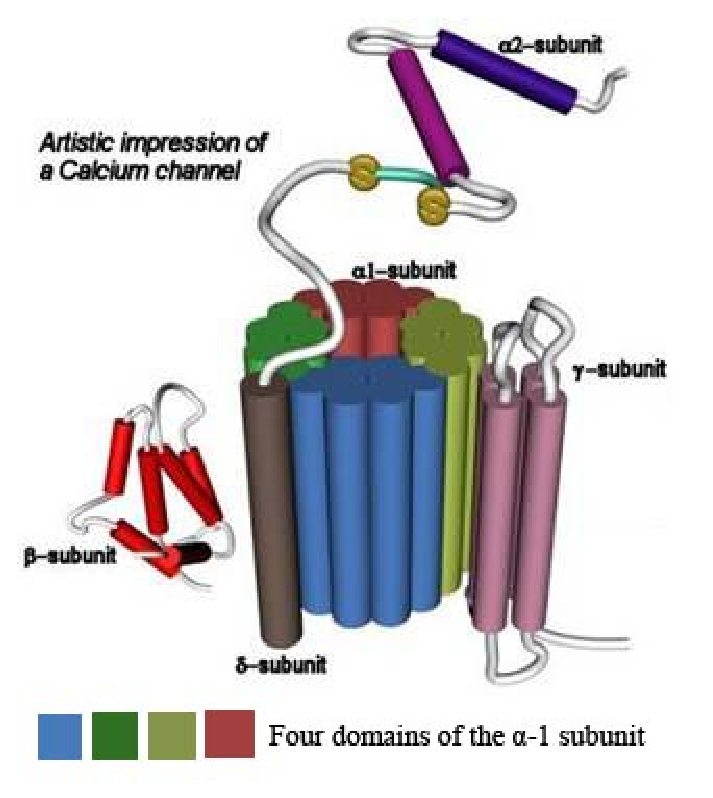
\includegraphics[height=7cm]{./images/Ca-channel-structure.eps}}
  \caption{Cartoon of the structure of a \ce{Ca^2+}
  channel\footnote{\url{http://www.sinc.sunysb.edu/Stu/glho/symptoms_clip_image002.jpg}}}\label{fig:ca_channel_structure}
\end{figure}

A calcium channel is in fact a complex transmembrane protein composed of 4 or 5
subunits, each is encoded by multiple
genes\footnote{\url{http://www.iuphar-db.org/IC/FamilyMenuForward?familyId=11}}.
$\alpha$ is the pore-forming subunit, and the others are auxiliary subunits.

\begin{enumerate}
\item {\bf $\alpha_1$ subunit} (Sect\ref{sec:alpha-1-subunit-VDCC}) : the largest subunit
  (190-250kDa). $\alpha_1$ subunit contains DHP binding site and most
  importantly form the pore of \ce{Ca^2+} channel.

This is the reason why $\Ca$ channel is aka DHPR (dihydropyridines receptor).

\item $\beta$ subunit (52kDa) (Sect.\ref{sec:beta-subunit-VDCC}): is the
intracellular subunit that regulate the activity of $\alpha_1$ subunit.

\item $\alpha_2\delta$ (160kDa) (Sect.\ref{sec:alpha-2-delta-subunit-VDCC}): is a transmembrane,
disulfide-linked complex ($\alpha_2$ subunit + $\delta$ subunit)

\item $\gamma$ subunit (32kDa) (Sect.\ref{sec:gamma-subunit-VDCC}): found mainly
in skeletal muscle cells, not in cardiac cells.
\end{enumerate}

\subsection[alpha-1 subunit]{$\alpha_1$ subunit}
\label{sec:alpha-1-subunit-VDCC}

Even though there are different subunits, however, the pharmacological and
electrophysiological diversity of \ce{Ca^2+} channels primarily arise from the
existence of multiple forms of the $\alpha_1$ subunit. Thus one way to classify
$\Ca$ channel is based on $\alpha_1$ subunit
(Sect.\ref{sec:calcium-channel-classification-alpha-subunit}).

An $\alpha_1$ subunit is
encoded by at least 10 distinct genes.
As shown in Fig.~\ref{fig:ca_channel_structure}, 
the subunit is organized in 4 homologous domain
(domain I - domain IV) , and 5 large intracellular
segments: N terminus (NT), C terminus (CT), and loops (L1,L2,L3) to links the
domains. 

Each domain contains 6 trans-membrane $\alpha$ helix segments (S1-S6) and a
re-entrant $p$-loop that is thought to contain the amino acids that line the
pore and form the selectivity filter \citep{catterall2005iup} with
\textcolor{red}{segment S4 is the voltage sensor}.
There are also a large number of short intracellular linkers between
transmembrane segments within each domain.

\begin{figure}[htb]
  \centerline{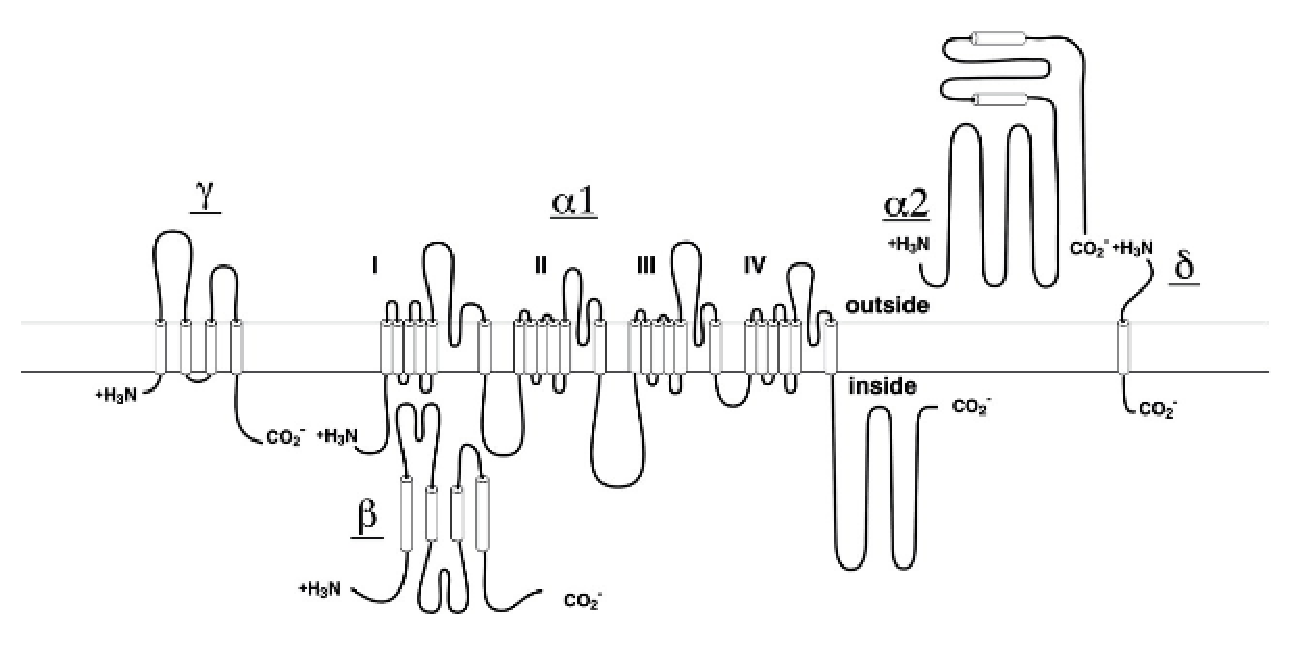
\includegraphics[height=7cm]{./images/Ca_subunit_structure.eps}}
  \caption{Subunit structure of Ca$_v1$ channels}\label{fig:ca_subunit}
\end{figure}

\subsection[beta subunit]{$\beta$ subunit}
\label{sec:beta-subunit-VDCC}

The $\beta$ subunit is the only calcium channel subunit for
which there is crystal structure information.
\begin{itemize}
  \item core of this subunit is homologous to membrane-associated guanylate
  kinases (MAGUKs), with a conserved interacting SH3 and guanylate kinase (GK)
  domains.
  
  Electrophysiological data showed that the co-expression of SH3 and GK domains
  is critical as either one of the regions along is incapable of regulating
  $\Ca$ channel activitity, i.e. showing the functional significance of the
  intramolecular SH3-GK interaction.
  
  
  \item residues on GK domain form a hydrophobic groove for high-affinity
  binding of HVA calcium channels.
\end{itemize}

\textcolor{red}{The mammalian brain expresses 4 different types of $\beta$
subunit}: $\beta_1$ through $\beta_4$, which can undergo alternate splicing.

They share a similar structural arrangement with two highly conserved regions
(C1 and C2) of high overall sequence homology (75\% and 85\%, respectively),
separated and flanked by 3 variable regions (V1 through V3) of much lower
homology (35-55\%).

A $\beta$ subunit physically binds to $\alpha_1$ subunit at
\begin{itemize}
  \item  a region within the $\alpha_1$ subunit domain I-II linker, highly
  conserved among HVA $\Ca$ channels. So they are called alpha interaction domain (AID).
  
  Binding of the $\beta$ subunit to AID region is critically dependent on
  functional association of the SH3 and GK region.
  
  \item report of a second calcium channel $\beta$ subunit interaction site
  within the C-terminus of $\alpha_1$ subunit, but the role of this site remain
  unclear.
\end{itemize}

Depending the subtype of $\beta$ subunit, it affects $\Ca$ channels kinetics,
and current densities. However, this is controversy as a recent study showed
that the calcium channel $\alpha_1$ subunit can give rise to robust current
activity even when expressed alone \citep{yasuda2004}.

The most obvious affect of $\beta$ subunit is on regulating channel {\bf
inactivation rates}
\begin{itemize}
  \item $\beta_{2a}$: dramatically slowing inactivation 
  \item $\beta_{3}, \beta_{1b}$: accelerate inactivation
\end{itemize}
(Review: \citep{kisilevsky2008})

\subsection[alpha-2-delta subunit]{$\alpha_2\delta$ subunit}
\label{sec:alpha-2-delta-subunit-VDCC}

There are four different types of calcium channel $\alpha_2-\delta$ subunit,
each is encoded by a single gene, and the two peptides $\alpha_2$ and $\delta$
are linked via a disulfide bond.

\subsection[gamma subunit]{$\gamma$ subunit}
\label{sec:gamma-subunit-VDCC}

The skeletal muscle L-type calcium channel complex also contains a $\gamma$
subunit ($\gamma_1$) which is a four transmembrane helix with cytoplasmic N- and
C-termini.

Seven additional potential candidates for neuronal calcium channel $\gamma$
subunits have been identified; however, it is not clear if these are bona fide
calcium channel subunits.
\begin{itemize}
  \item The association of $\gamma_2$ and $\gamma_3$ to neuronal $\Ca$ channels
  \citep{kang2001, letts1998}

  The neuronal $\Ca$ channel $\gamma_2$ subunit (stargazin) has also been linked
  to AMPA receptor trafficking and pharmacology. Stargazin functions as a
  chaperon protein for proper folding and
surface expression of AMPA receptors (Sect.\ref{sec:AMPAR}).
Stargazin also involves
in the synaptic targeting of AMPA receptors through its interaction
with PSD95, a scaffolding protein enriched in postsynaptic
density (PSD).
  
\item 
\end{itemize}


\section{Nomenclature}
\label{sec:nomenclature-Cav-channels}

We use the parallel nomenclature for ion channel called UCL/HGNC/HUGO Human Gene
Nomenclature symbols which is developped in conjunction with the human genome
project (reference: Sect.\ref{sec:nomenclature-K_channel},
Sect.\ref{sec:nomenclature-Na-channel}) - review: Trimmer, Rhodes (2004).

However, the scenario for $\Ca$ channels are more disorganized and more complex
\begin{enumerate}
  \item Cav1.1 (need $\alpha_{1S}$) is CACNA1S
  
  \item Cav3.1 (need $\alpha_{1G}$) is CACNA1G
\end{enumerate}


\subsection{Based on alpha-subunit ($\alpha$-1S, $\alpha$-1A, $\alpha-$1B,
$\alpha-$1F)}
\label{sec:calcium-channel-classification-alpha-subunit}
\label{sec:alpha-subunit-Ca2+channel}

Historically, there are various names given to the corresponding gene products
$\alpha_1$. In 1994, a unified nomenclature was adopted - $\alpha_1$ subunits
were referred to as 
\begin{itemize}
  \item  $\alpha_{1S}$ for the original skeletal muscle isoform (S=skeletal) 

  \item $\alpha_{1A}$ to $\alpha_{1E}$ for those discovered subsequently.
%   \begin{itemize}
%     \item $\alpha_{1C}, \alpha_{1E}$: found in cardiac cells 
%     
%   \end{itemize}
  
  \item  Since then, there are 4 new $\alpha_1$ subunits have been identified,
  i.e. $\alpha_{1F}$, $\alpha_{1G}, \alpha_{1H}, \alpha_{1L}$.
  
\end{itemize}


\subsection{Based on numerical system (Cav1, Cav2, Cav3)}
\label{sec:Cav1.x}
\label{sec:Cav2.x}
\label{sec:Cav3.x}

As $\alpha_1$ is the pore-forming subunit, the genes encoding this subunit is
often used to classify the ion channel. The genes encoding $\alpha_1$ subunits
fall into 3 families using numerical system, Fig.\ref{fig:Ca_channel_info}:
\begin{itemize}
  \item Cav1 (Ca$_v$1): encode 4 different L-type $\Ca$ channel isoforms
  (Cav1.1-1.4) - Sect.\ref{sec:L-type-Ca2+}.
  
  In mammal, Cav1.1-1.4 are encoded by $\alpha$1 subunit genes CACNA1S, CACNA1C,
  CACNA1D, and CACNA1F respectively. 
  
  Cav1-type calcium channels are sensitive to dihydropyridine (DHP) antagonists
  such as nifedipine or nimodipine, or to phenylalkylamines like verapamil; so
  they are aka DHPR channels in cardiac cell. They are thus aka DHPR, i.e.
  DHP-receptor.
  
  \item Cav2 (Ca$_v$2): encode three different (intermediate)-threshold
  activated calcium channels:  N-type, splice variant P/Q-type, and R-type $\Ca$
  channels.
  
  At the neuronal synapse: P/Q-type (Cav2.1), N-type (Cav2.2), R-type (Cav2.3) -
  Sect.\ref{sec:R-type_Ca-channel}
  
  \item Cav3 (Ca$_v$3): encode 3 different low-threshold activated calcium
  channels T-type $\Ca$ channel isoforms: T-type (Cav3.1-3.3) = LVA
  (low-voltage activated)
  
\end{itemize}
Except T-type, all other types are HVA (high-voltage activated) -
Sect.\ref{sec:HVA_Ca2+}.

\begin{figure}[hbt]
  \centerline{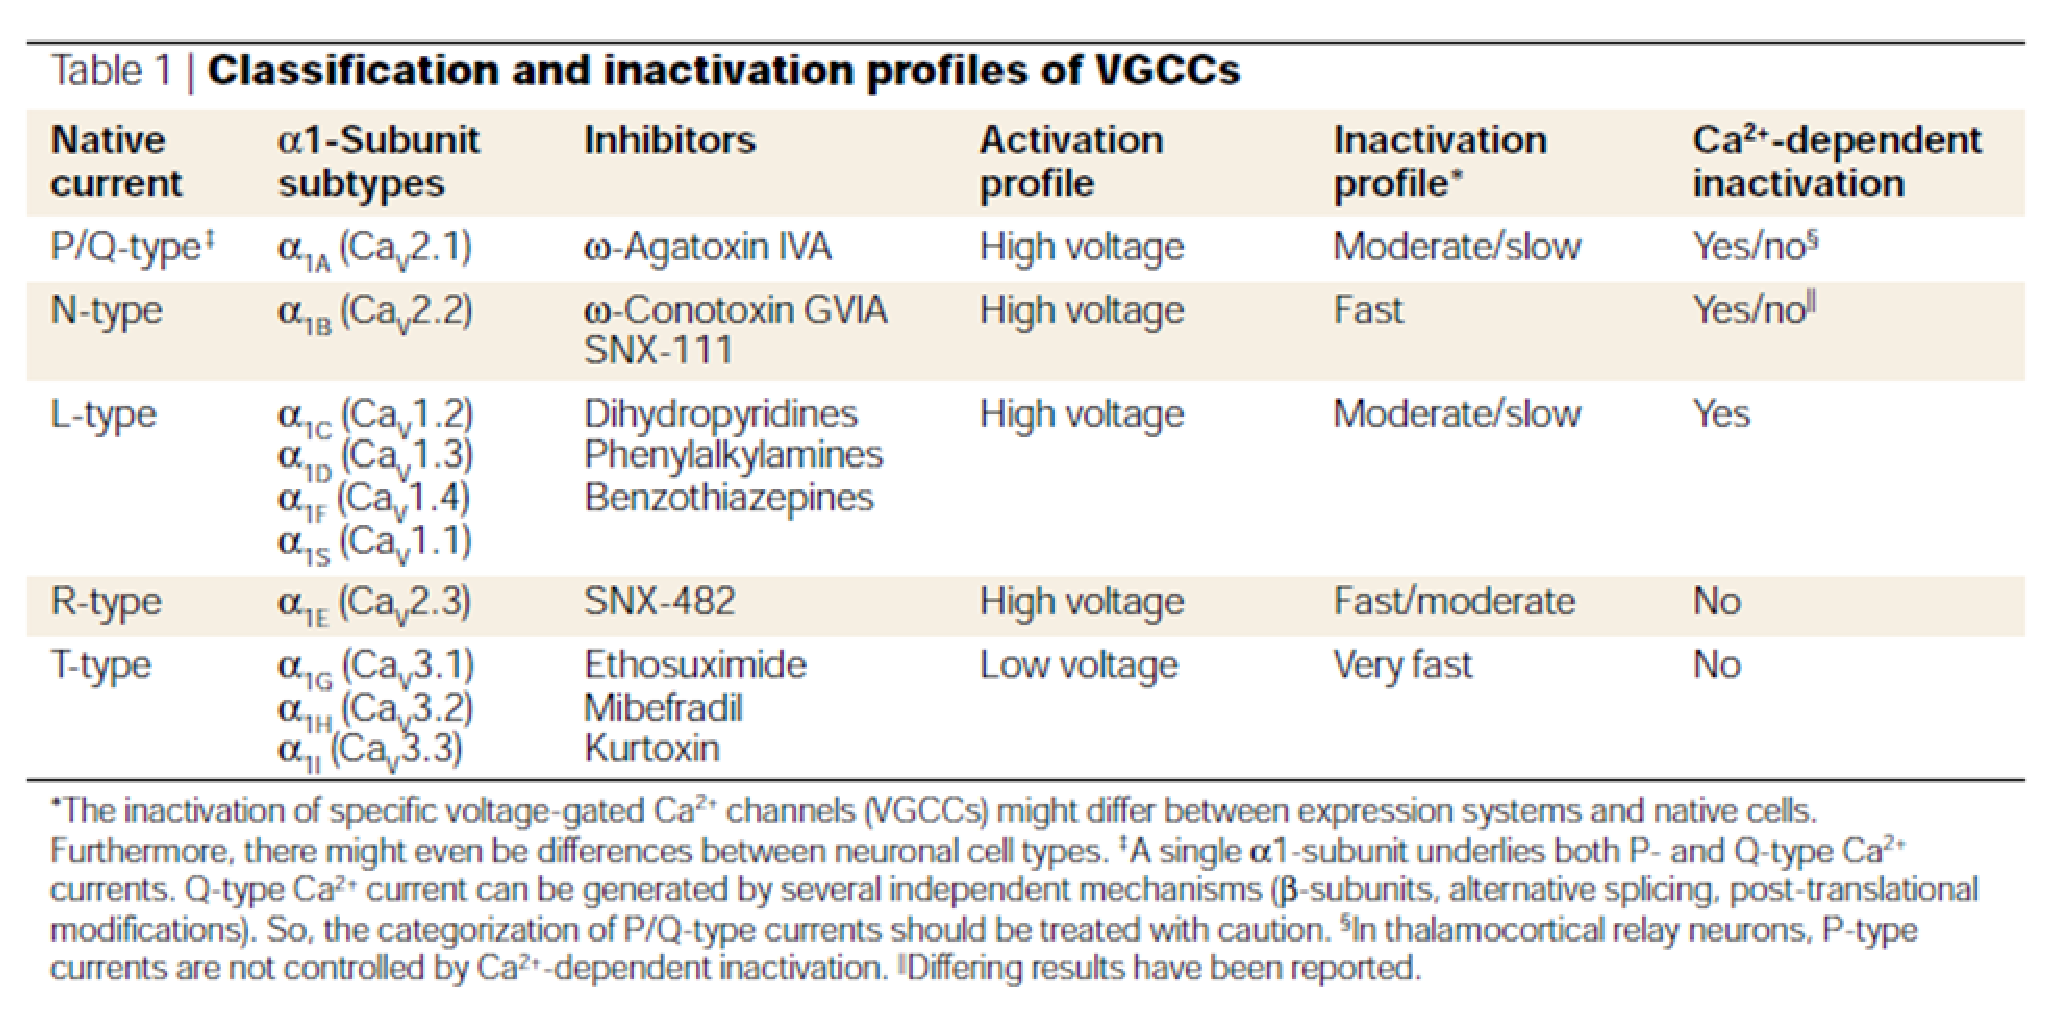
\includegraphics[height=6cm,
    angle=0]{./images/Ca_channel_info.eps}}
\caption{Classification and inactivation profiles of $\Ca$ channels}
\label{fig:Ca_channel_info}
\end{figure}


In 2000, a rational nomenclature was adopted based on the well-defined $\alpha$
subunit of potassium channels \citep{Ertel2000Nomenclature}
(Chap.\ref{chap:potassium-channels}). This nomenclature uses a
numerical system (Ca$_v1.1$, Ca$_v2.1$,Ca$_v3.1$, etc.) to define families and subfamilies of
\ce{Ca^{2+}} channels based on similarities in amino acid sequences,
as shown in Fig.~\ref{fig:ca_channel_phylogeny}
\citep{catterall2005iup}.

\begin{figure}[htb]
  \centerline{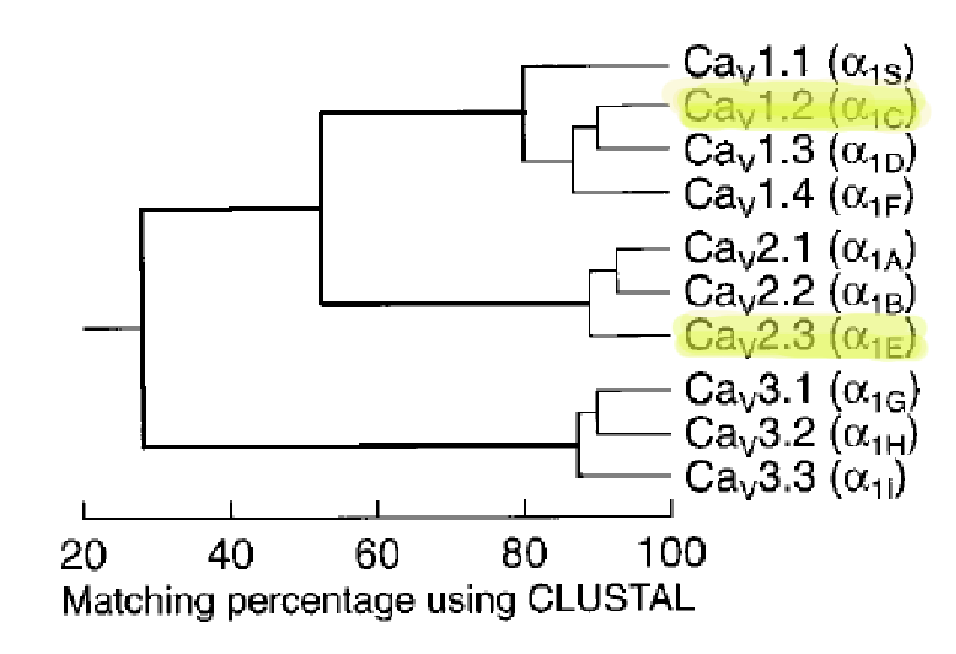
\includegraphics[height=5cm]{./images/Ca_channel_nomenclature.eps}}
  \caption{Phylogeny of \ce{Ca^2+} channels $\alpha_1$ subunits}
  \label{fig:ca_channel_phylogeny}
\end{figure}

\subsection{Based on voltage-dependent (LVA, HVA)}
\label{sec:LVA_Ca2+}
\label{sec:HVA_Ca2+}

Remembering that the movement of ions cause an electrical current.
Correspondingly, the flow of \ce{Ca^2+} through a \ce{Ca^2}-channel on the
plasma membrane cause an electrical current $I_{\Ca}$ whose magnitude can be used
to represent a calcium ion channel. Hence, an alternate naming system ($I_{\Ca}$)
is used based on the level of depolarization of voltage:
\begin{itemize}
  
  \item  {\it low-voltage-activated calcium channels} (LVA): display rapid
  gating kinetics, exhibit a small unitary conductance, and play a major role in
  neuronal pacemaker activity (T-type $\Ca$ channels) -
  Sect.\ref{sec:T-type_Ca-channels} (Akaike, 1991; Huguenard 1996).

  \item {\it high-voltage-activated calcium channels} (HVA): require more
  positive membrane depolarization in order to open and can be further
  categorized, based on their functional characteristics, into N-, P-, Q-, R-,
  and L-types (see next classification scheme). - Sect.\ref{sec:HVA_Ca2+} (Bean,
  1989).

HVA is classified into 
\begin{enumerate}
  \item HTS = high-threshold sustained component
  
  \item HTI = high-threshold inactivating component
\end{enumerate}


\end{itemize}

\subsection{-- HVA: HTS, HTI}
\label{sec:HTS-HVA-Ca2+-current}
\label{sec:HTI-HVA-Ca2+-current}

Chirchill, MacVicar (1998) 

\subsection{Based on alphabetical system (L-type, P/Q-type, R-type, T-type)}
\label{sec:calcium-channels-classification-alphabet}
\label{sec:L-type-Ca2+}
\label{sec:P/Q-type-Ca2+}
\label{sec:T-type-Ca2+}
\label{sec:CaL-type}

Finally, the third nomenclature is to use an alphabetical system.

\begin{itemize}

  \item L-type: LCC = L-type $\Ca$ channels  (L=long-lasting (i.e. the channel
  activate later and last longer)) - Sect.\ref{sec:DHPR-Ca2+channel}

There are 4 different L-type $\Ca$ channels; encoded by $\alpha_{1C}$ and
$\alpha_{1D}$ genes (Sect.\ref{sec:alpha-subunit-Ca2+channel}).

$\alpha_{1D}$ is expressed at relatively high levels in pacemaker cells.
In ventricular myocytes, L-type \ce{Ca^2+} channel ($I_{Ca,L}$) derived from
$\alpha_{1C}$ is dominant and is the main concern.

$I_{Ca,L}$ derived from $\alpha_{1D}$ activates at an intermediate potential
($V_m$) between that for $I_{Ca,T}$ and $I_{Ca,L}$ derived from $\alpha_{1C}$.
Eventually, $I_{Ca,L}$ and $I_{Ca,T}$ serve different functional role.


  \item N-type (`N' for Neural-type): found mainly pre-synaptic terminals and
  involve in neurotransmitter release. Strong depolarization by an AP causes
  these channels to open and allow influx of \ce{Ca^2+}, initiating vesicle
  fusion and release of stored neurotransmitter.

N-type is encoded by Cav2.1 gene ($\alpha$1A subunit), which can be identified
using Cav2.1 antibody.

\begin{mdframed}
NOTE: $\alpha_\text{1C}$ is the pore-forming subunits of L-type; while
$\alpha_\text{1A},\alpha_{1B}$ are the pore-forming subunits of P/Q-type and
N-type, respectively.
\end{mdframed}

  \item P-type (`P' for Purkinje cells): found mainly in Purkinje fibers in the
electrical conduction system in the heart. They functions as N-type channels 

P/Q-type is encoded by Cav2.2 gene ($\alpha$1B subunit), which can be identified
using Cav2.2 antibody.
 
  \item Q-type: poorly understood. They has a high threshold of
  activation and relatively slow kinetics. 

  \item R-type: poorly understood. They has a high threshold of
  activation and relatively slow kinetics. 

  \item T-type: produce pacemaker potential in the SA node of the heart.
(T = transient (i.e. the channel activate early and inactivate soon after
that))

T-type channels are encoded by $\alpha_{1G}$ and $\alpha_{1H}$ genes
(Sect.\ref{sec:alpha-subunit-Ca2+channel}).
T-type means transient low-threshold voltage activated $\Ca$ current, activated
at potential ranging -50mV to -30mV and display fast inactivation.

\end{itemize}

\subsection{-- T-type (Cav3.1, Cav3.2, Cav3.3)}
\label{sec:T-type_Ca-channels}

In the heart, T-type $\Ca$ channel was detected in atrial \citep{bean1985} and
ventricular \citep{nilius1985}. This channel activate and inactivate at the potential
($<-50$mV) far negative below the range for activating L-type $\Ca$ channels. 
\textcolor{red}{T-type channels activate earlier than L-type and also
inactivate completely at $V_m < -50$mV} \citep{hess1984}. 

\begin{framed}
  T-type channels activate at a more negative potential and also
  inactivates more rapidly than L-type channels. T-type channels resides
  mainly at conducting system (His bundle, Purkinje cells) and pacemaker
  cells, while L-type channels are dominant in non-pacemaker cells, e.g.
  myocardial cells (ventricular myocytes). The only exception with which
  $I_{Ca,T}$ is found in ventricular myocytes is adolescent with
  immature and developing hearts~\citep{chen2007afh}; yet the current is
  still small compared with $I_{Ca,L}$.
  \textcolor{red}{Hence, it is clear that L-type (from $\alpha_{1C}$) is
    responsible for EC coupling in cardiac myocytes.}
\end{framed}

\subsection{-- L-type ($I_{Ca,L}$)}
\label{sec:L-type_Ca-channels}

L-type means long-lasting and later-activated, i.e. high-threshold voltaged
$\Ca$ current. Its first detected blocker is dihydropyrinidine (i.e.
nifedipine), so the channel is also known as {\bf dihydropyrinidine receptor
(DHPR)} \citep{reuter1985}. Other blockers: cadmium (\ce{Cd^2+}) so the current
is aka called $\Cd$-sensitive $\Ca$ current.

$I_{Ca,L}$ involves in contraction of heart muscle, gene expression in
neurons, hormone secretion, etc.
\textcolor{red}{So, whenever we're talking about $I_{Ca,L}$, it is
  about L-type from $\alpha_{1C}$}.


In {\bf cardiac cells}, LCC (expressed by $\alpha$-1C gene) is an essential
transmembrane ion channel that serves 2 main functions: (1) trigger the
initiation of excitation contraction (EC) process, (2) generate the prolonged
depolarization characteristic of cardiac AP.

In {\bf neurons}, LCC is accepted that voltage-dependent facillitation is
PKA-dependent as it's sensitive to $\beta$-adrenergic stimulation
\citep{hadley1991} (Sect.\ref{sec:beta-adrenergic_stimulation}), not G
protein-dependent.
However, there was evidence that G$\beta\gamma$ can also reduce current, though
the physiological role was unclear \citep{ivanina2000}.
The data by \citep{hoogland2004} suggested that LCC are functionally present in
dendritic spines of CA1 pyramidal neurons, contribute to spine Ca2+ influx, and
can be modulated by the $\beta_2$ adrenergic receptor through PKA in a highly
compartmentalized manner.




\subsection{Based on the inhibitor (DHPR)}
\label{sec:DHPR-Ca2+channel}

Another less common use to distinguish \ce{Ca^2+} channels are based
on their inhibitors. 
\begin{itemize}
\item L-type \ce{Ca^2+} channels is blocked selectively by some
  antagonist, e.g.  1,4-dihydropyridines (DHPs), phenylalkylamines,
  and benzothiazepines.  
  
  \textcolor{red}{L-type channels on T-tubules of the cardiac
  myocytes are blocked by DHP, and thus are called DHP receptors
  (DHPR).}

  Even though N-type, P/Q-type and R-type calcium channels are all
  HVA calcium channels, they are relatively unaffected by L-type calcium channel
  antagonist drugs, as described above, but are blocked by specific toxins from
  snails and spider venoms (see below).

  \item N-type  \ce{Ca^2+} channels generated by Ca$_v2.2$ is block selectively
by $\omega-$conotoxin GVIA, MVIIA, and CVID.

  \item P- and Q-type channels are differentially sensitive to $\omega$-agatoxin
IVA.
  
  \item R-type channels have shown to be potently inhibited by the spider toxin
  SNX-482.
  
\item T-type calcium channels are classified as LVA, i.e. weak
  depolarization and are transient. They are resistant to both organic
  antagonists and to the snake and spider toxins as described above.

\end{itemize}

\section{Distribution of $\Ca$ channels}
\label{sec:calcium-channels-distribution}

So, we have learnt different types of \ce{Ca^2+} channels and
different naming systems. In addition, different types of
voltage-gated calcium channels are spatially distributed differently
in variety types of cells.  
\begin{itemize}
\item L-type \ce{Ca^2+} from $\alpha_{1C}$ is mainly found in cardiac
  myocytes, smooth muscle cells, endocrine cells, neuronal cell bodies
  (support $\Ca$-dependent gene transcription) and proximal dendrites.  
  
  As the ventricles are the chambers that are major component of EC coupling, it
  is L-type \ce{Ca^2+} from $\alpha_{1C}$ that mediate EC coupling in skeletal,
  cardiac and smooth muscles.
  \textcolor{red}{Later on, when referring to L-type channels, it
    means L-type \ce{Ca^2+} channels from $\alpha_{1C}$.}
  

\item L-type \ce{Ca^2+} from $\alpha_{1D}$ is
  present in cardiac atrial myocytes, pacemaker cells, endocrine cells, neuronal
  cell bodies and dendrites.
  

\item N-, P/Q- type \ce{Ca^{2+}} channels (Sect.\ref{sec:N-and-P/Q-type}) are
expressed prominently in neurons, particularly presynaptic nerve terminals
(control evoked neurotransmitter release).

On the presynaptic nerve terminal, strong depolarization by an action potential
causes these channels to open and allow influx of Ca2+, initiating vesicle
fusion and release of stored neurotransmitter.

\begin{enumerate}
    \item N-type are found in soma, dendrites and a subpopulation of dendritic
  spines (tested on CA1 region of rat hippocampal slices \citep{mills1994})
  
  \item P/Q-type are found in Purkinje fiber with two distinct patterns
  (scatter and clustered) \citep{indriati2013}:
  scater = increasing 2.5-fold from soma to distal dendrites, clustered (74-fold
  higher density than the scattered particles) = on the P-face of soma and
  primary dendrites.
  
  The clustered P/Q-type were found virtually colocalize with 2 types of
  calcium-activated potassium channels, BK and SK2, with the nearest neighbor
  distance of $\sim$ 40 nm.
  
\end{enumerate}

 \item R-type (Sect.\ref{sec:R-type_Ca-channel}) have been found to play a role
 in evoked neurotransmitter release in certain synapses
 
  N-type ($\alpha_\text{1B}$) and P/Q-type
 ($\alpha_\text{1A}$)) , and other cells (R-types
 - ).

\item T-type calcium channels can be found in a wide variety of cell
  types, where they are involved in shaping the AP and controlling
  patterns of repetitive firing.

Single-channel recordings from guinea pigs suggest that T-type channels are
particularly abundant on hippocampal CA3 pyramidal neurons, as compared with
neurons from area CA1 or the dentate gyrus (Fisher et al., 1990).

\end{itemize}
\textcolor{red}{In heart, we often see Ca$_v1.2$} ($\alpha_{1C}$, L-type) and
\textcolor{red}{Ca$_v2.3$.} ($\alpha_{1E}$, R-type); while Ca$_v1.1$
($\alpha_{1S}$) is found in skeletal muscle.

In cardiac myocytes, calcium channels are particularly abundant in the
transverse (T)-tubule system and they are L-type Ca channels (LCCs) 
which are also classified as HVA, is generated by Ca$_v1.2$ ($\alpha_{1C}$) or
Ca$_v1.3$ ($\alpha_{1D}$). Guinea pig ventricular cells show 2 distinct types of $\Ca$
channel: L-type and T-type. L-type ($\alpha_\text{1C}$) is dominant in
ventricular myocytes.


% L-type DHPR channels is a type of voltage-gated \ce{Ca^2+} channels
% found mainly in cardiac myocytes and mediate calcium influx in
% response to membrane depolarization.  However, the low-level entry
% \ce{Ca^2+} is not enough to cause contraction in myocytes. It is the
% release of \ce{Ca^2+} from intracellular stores \citep{bassani1995fsr},
% in which the elementary event is termed
% {\bf
%   \ce{Ca^2+}-sparks}\footnote{\ce{Ca^2+}-sparks
%   is a large transient increase of localized internal [\ce{Ca^2+}]
%   from a group of RyRs and will be discussed in detail in
%   Chap.~\ref{chap:calcium-signalling}}. The free \ce{Ca^2+} in the
% myoplasm then regulate intracellular
% processes\footnote{
%   {\it e.g. excitation-contraction coupling (ECC),
%     excitation-secretion coupling, neurotransmission},
%   and {\it gene expression}, depending on the types of cells}.
% 

% 
% \section{T-type vs. L-type}
% \label{sec:T-and-L-type_Ca-channels}
% \label{sec:calcium-current}
% 
% L-type calcium current refers to the transportation of \ce{Ca^2+}
% through the ventricular sarcolemma (plasma membrane of ventricular
% myocytes) via L-type calcium channels.  $I_{Ca,T}$ is LVA
% (low-voltage-activated) while $I_{Ca,L}$ is HVA. Hence, $I_{Ca,T}$ is
% more independent of \ce{Ca^2+} influx.  
% 
%  while

%\subsection{L-type}

\section{L-type, Cav1.2 ($\alpha$)}
\label{sec:CaLv1.2-channel}

Unlike CaLv1.3 channel, CaLv1.2 is a HVA calcium channel
(Sect.\ref{sec:HVA_Ca2+}).



\subsection{$I_{Ca,L}$ activation}
\label{sec:i_ca-l-activation}


\begin{figure}[htb]
  \centerline{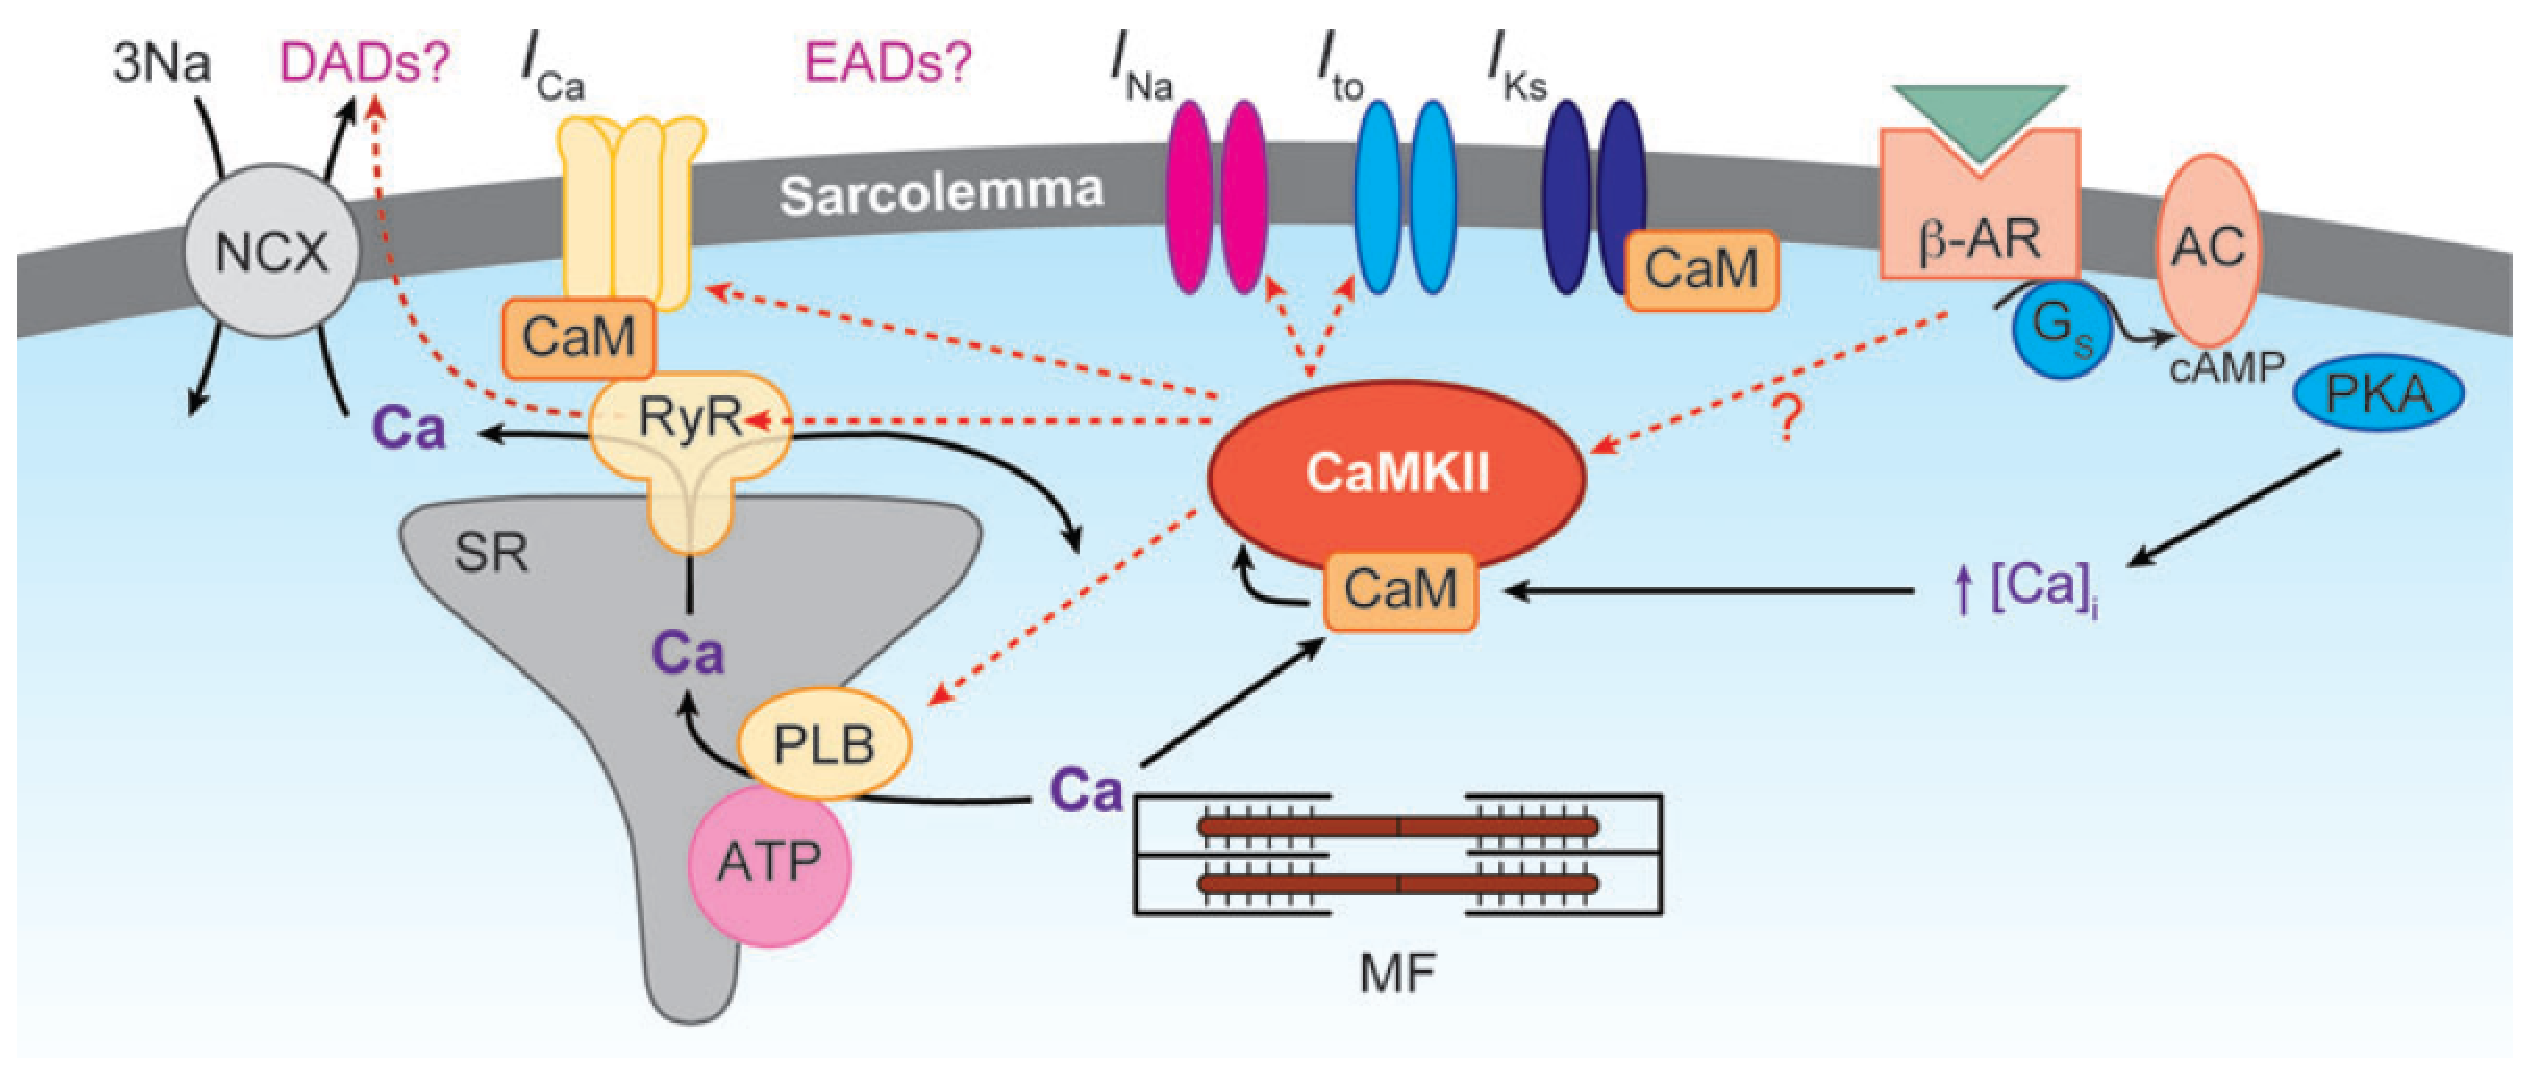
\includegraphics[height=5.5cm]{./images/Ca_cycling.eps}}
  \caption{\ce{Ca^2+} cycling}\label{fig:Ca_cycling}
\end{figure}

In addition to the $V_m$-dependent activation of L-type current, in
cardiac myocytes, the facilitation for $I_{Ca,L}$ is found to depends
on {\bf \ce{Ca^2+}/CaM-dependent protein kinase II}
(CaMKII)\footnote{\url{http://openwetware.org/wiki/BIO254:CaMKII}}. 

CaMKII is activated when the complex \ce{Ca^2+}/CaM bind to it. The activation
of CaMKII can facilitate the activation of \ce{Ca^2+} channels. This happens
over a longer timescale (from one beat to the next) and as a result increase
$I_{Ca,L}$ amplitude.
\textcolor{red}{The molecular mechanism is not fully resolved}.


\subsection{$I_{Ca,L}$ inactivation}
\label{sec:calcium-inactivation}

Opposing to the activation process, there is a process that decreases
$I_{\ce{Ca},L}$.
\textcolor{red}{During AP, $I_{Ca,L}$ turnoff is mediated by both
  voltage- and \ce{Ca^2+}-dependent inactivation, yet the latter is by
  far predominant}~\citep{bers2001ecc}.
Indeed, the \ce{Ca^2+}-dependent inactivation is expressed via
{\bf calmodulin} (CaM), the classical \ce{Ca^2+} receptor protein
inside cells. Several studies concluded that {\bf calmodulin} (CaM)
mediates both inactivation and
facilitation~\citep{lee1999calm, zuhlke1999calm}.
\textcolor{red}{However, the question is how CaM act to inactivate
  LCC},
e.g. it binds directly to the LCC or indirectly by interacting with
some protein kinases or phosphatases to regulate the LCC?.
~\citep{ehlers1999calm} proposed 3 models,
Fig.~\ref{fig:calmodulin_hyp}, with a tether site (IQ-motif) for CaM
constitutively bound under resting condition, as well as a
CaM-effector site through which \ce{Ca^2+}-associated CaM
(\ce{Ca^2+}/CaM) modulate channel gating.

\begin{figure}[hbt]
  \centerline{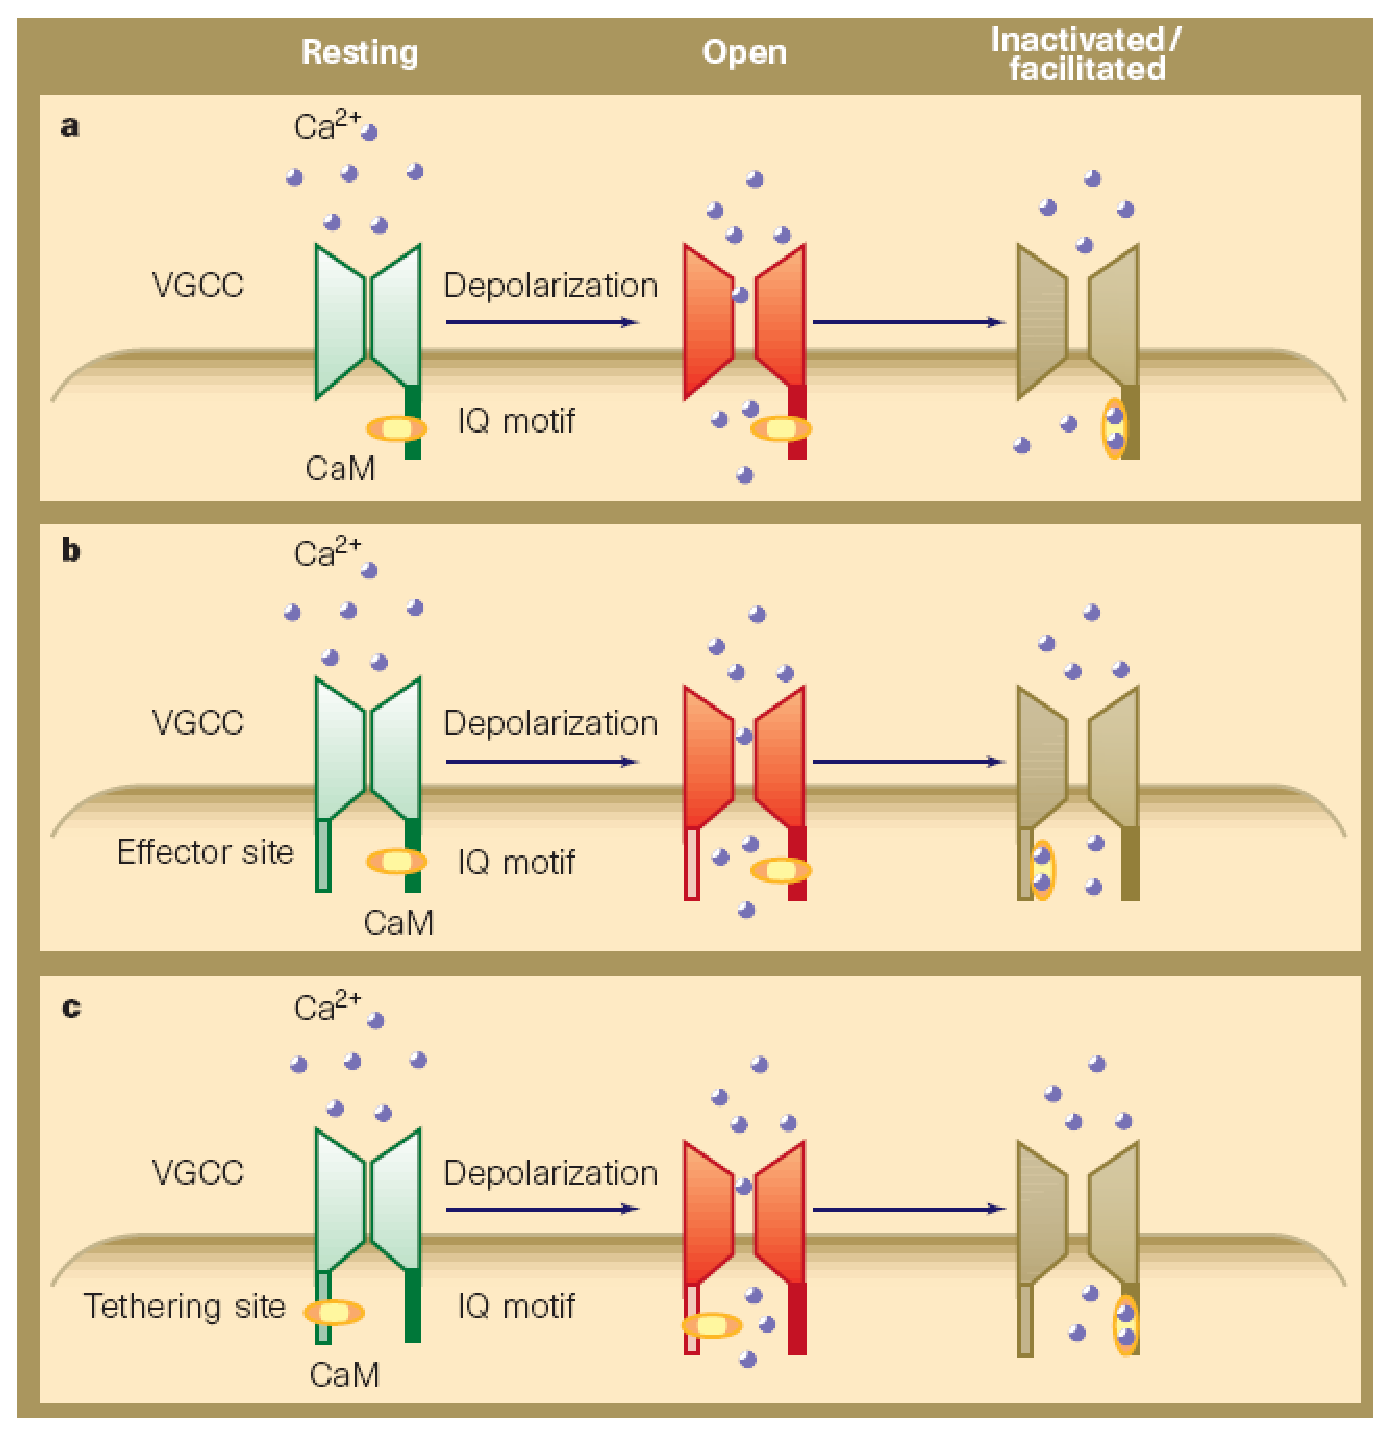
\includegraphics[height=7cm,
    angle=0]{./images/calmodulin_inactivation.eps}}
  \caption{Three different models for Calmodulin (CaM) inactivation of
    voltage-gated calcium channels (VGGC): (A) IQ-motif acts as both
    tether and effector, (B) IQ-motif acts as effector only, (C) tether only}
  \label{fig:calmodulin_hyp}
\end{figure}

With an increase in $[\ce{Ca^2+}]_{ds}$ (owing to the influx of
calcium or release from SR), it triggers the activation of CaM - a
protein activated when bind with \ce{Ca^2+}. Activated CaM - known as
Ca2+/CaM complex, can associate with the C terminus of the $\alpha_{1C}$
protein ({\it read a Chapter in Cardiology book}).  Precisely, Ca2+/CaM
binds to an IQ-like motif (isoleucine-glutamine) (or EF-hand) on the
carboxyl tail on the main
$\alpha_{1C}$-subunit~\citep{zuhlke1999calm}.
 
\begin{framed}
  An IQ motif is an extremely basic unit (23 amino acids) that serves
  as a binding site for different EF-hand proteins (e.g. myosin light
  chain, CaM, CaM-like proteins). Many IQ motif are protein kinase C
  (PKC) phosphorylation sites. 
\end{framed}

The electrical stimuli will depolarize the membrane voltage difference
$V_m$ at the T-tubules of cardiomyocytes. The depolarization will open
some LCCs.  When the potential difference passes a threshold, it can
trigger/cause/activate enough number of LCCs from which the Ca influx
can induces the release of Ca form internal calcium storage (SR) via
RyR channels. This is a process known as CICR and the transient
increase in internal [Ca] lead to the transient depolarization in
membrane potential. The transient increase in myoplasmic [Ca] can
trigger some subcellular events (an action), hence we call this
transient depolarization in membrane potential is an
{\bf action potential} (AP).

In summary, the \ce{Ca^2+}-dependent $I_{Ca,L}$ inactivation may
function as a negative feedback system to limit \ce{Ca^2+} influx
under conditions in which \ce{Ca^2+} influx and SR \ce{Ca^2} release
is high. This can be a protection against cellular \ce{Ca^2+}
overload, which can cause arrhythmias and cell death. $I_{Ca,L}$
facilitation may serve to offset the negative effect of increased
frequency on \ce{Ca^2+} channel availability. Lastly, the amount of
\ce{Ca^2+} influx via $I_{Ca,L}$ during AP varies among cell types.

\section{L-type, Cav1.3 ($\alpha$)}
\label{sec:CaLv1.3-channel}

CaLv1.3 channels is a LVA calcium channel (Sect.\ref{sec:LVA_Ca2+})

\section{N-type and P/Q type}
\label{sec:N-and-P/Q-type}

N-type and P/Q-type are neuronal voltage-dependent $\Ca$ channels.
P/Q- and N-type channels trigger synaptic transmission in the majority of
neurons of the central nervous system. 

However, whether and under which conditions both channel types act cooperatively
or independently is still insufficiently understood.
A recent study suggested a more direct coupling of P/Q type to synaptic release
compared to N-type \citep{nimmervoll2013}.


These channels are inhibited by neurotransmitters (a voltage-independent
pathway) and voltage-repolarization. 
\begin{itemize}
  \item  In the voltage-independent pathway, the channels are
usually inhibited by G protein-coupled receptors
(Sect.\ref{sec:G-protein-coupled-receptor} via several second messenger
pathways.
  \item The voltage-dependent mechanism of N-type and P/Q type is G protein-dependent,
which is the result of a direct binding of G$\beta\gamma$ subunit G protein to
the channel. 

G-beta-gamma (G$\beta\gamma$) complex is a dimeric protein complex which is
cleaved from the G$\alpha\beta\gamma$ complex upon the activation of G-protein
coupled receptor. This allow the G-alpha (G$\alpha$) to function as a messenger
in signal transduction (Sect.\ref{sec:G-protein}). As the matter of fact, the
role of G$\beta\gamma$ is to inhibit G$\alpha$ subunit. However, the free
G$\beta\gamma$ has also found to play a role in other cellular activities; one
of that is L-type calcium channel \citep{dupre2009}.

\end{itemize}


\section{R-type $\Ca$ channels}
\label{sec:R-type_Ca-channel}

The R-type calcium channel is a type of voltage-dependent calcium channel
(Sect.\ref{sec:calcium-channels-classification-alphabet}), and is strongly
expressed in cortex, hippocampus, striatum, amygdala and interpeduncular nucleus
of the brain.

They have a high threshold of activation and relatively slow kinetics.
They are poorly understood, but like Q-type calcium channels, they appear to be
present in cerebellar granule cells. 

\section{Reconstituted $\Ca$ channels}
\label{sec:reconstitute_LCC}

To study single channel kinetics, it's important to extract the protein from the
media. Since 1989, the LCC channel was purified from rabbit skeletal muscle
T-tubules and then incorporated into phospholipid bilayer membranes at the tip
of glass patch pipettes~\citep{mcdonald1989}. The solution on both sides of the
bilayer contained (in mM): \ce{BaCl2} 90, HEPES 5, TTX 0.02 (pH 7.3 at
20-23$^\circ$C).


\section{$\Ca$ current on}
\label{sec:calcium-current-on}

\subsection{Squid giant axon }
\label{sec:calcium-current-on-axon}

$\Ca$ entry through squid axon membrane has been shown as 2 components
\begin{itemize}
  \item early component as a leak of $\Ca$ ions through TTX-sensitive $\Na$
  channels
  
  \item a late component which is not affected by TTX
\end{itemize}
The amount of Ca entering the fibre is very small, i.e. 0.08 pM/cm$^2$ per AP
with 112 mM $\Ca$ in external solution (represents a charge transfer 0.02
$\mu$C/cm$^2$), compared to net $\Na$ entry 3-4 pM/cm$^2$ (represents a charge
transfer 0.3-0.4 $\mu$C/cm$^2$) \citep{meves1973cic}.

In squid giant axon, the calcium current was activated at about -40 mV and it
peaked at about 0 mV. The peak inward current was 3 microA/cm2 when external Ca
was 80 mM and 0.9 microA/cm2 in 8 mM Ca \citep{dipolo1983}.
In 80 mM Ca, the calcium current is turned on in less than 10 msec, and it does
not decay appreciably for pulses up to 70 msec in duration.

Barium can replace calcium, and cadmium blocks the calcium current
(Sect.\ref{sec:cadmium}).

\section{Signal detection}

Early efforts of measuring $I_\CaL$ {\it in vivo} using optical imaging
techniques involved using aequorin (Sect.\ref{sec:aequorin}). Voltage-clamped
protocol is often used to measure $I_\CaL$, with the ability to control the
level and duration of membrane depolarization, which cannot be obtained using
action potential (AP). The interpretation of aequorin signal can be complicated
as the elevation of aequorin signal can be the result of $I_\CaL, I_\NCX$ or the
release of $\Ca$ from calcium internal storage.

\begin{enumerate}
  \item Aequorin signals were sampled at 0.5ms interval; then filtered with an
  exponential filter of 2ms. The final output is the average of about 100
  aequorin signals \citep{wier1982}.
\end{enumerate}

\begin{figure}[hbt]
  \centerline{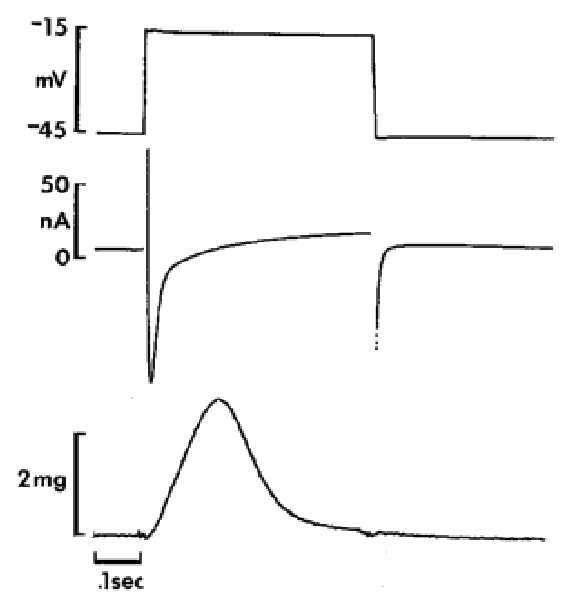
\includegraphics[height=5cm]{./images/LCC_current_Purkinje.eps}}
  \caption{Purkinje fibre (from top to bottom): Membrane potential, LCC current
  and tension (derived from \citep{wier1982}). The peak tension reached at 140ms after the
  starting of voltage clamp depolarization; relaxation starts after 400ms}
  \label{fig:LCC_current_Purkije_Wier82}
\end{figure}

Read more: Sect.\ref{sec:unit-i_cal-curr}, Sect.\ref{sec:IcaL_macroscopic}

\subsection{Density}

Early estimate of LCC density shown that about 0.5-5 channels/$\mum^2$
\citep{reuter1984}. Based on whole-cell current, it's estimated about
$10^4-10^5$ channels per cell (of medium size or total capacitance $C_m\sim
150$pF).

\subsection{$P_o$}

\begin{figure}[hbt]
  \centerline{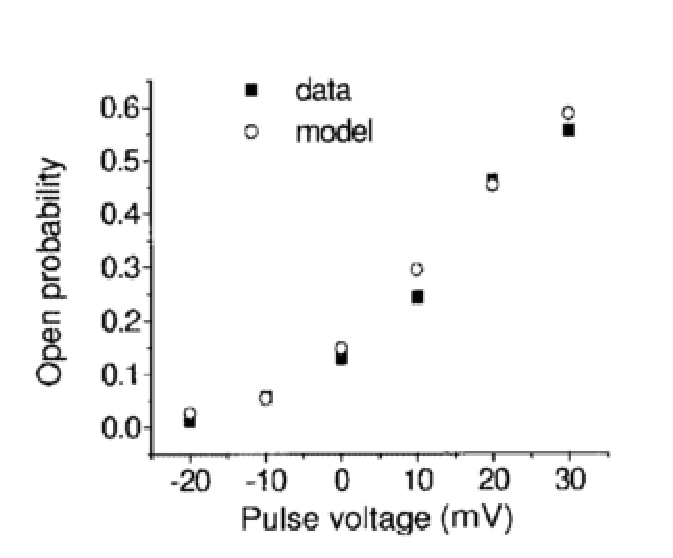
\includegraphics[height=5cm,
    angle=0]{./images/LCC_Po_Sun2000.eps}}
  \caption{The opening probability $P_o$ at different voltage clamp using $\Ba$
  as charge carriers, $[\Ba]_o=100$mM \citep{sun2000mlc}}
  \label{fig:LCC_Po}
\end{figure}

The probability of opening $P_o$, Fig.\ref{fig:LCC_Po} are estimated using
different methods:
\begin{enumerate}
\item with high $[\Ba]_o$, substituting for $\Ca$, as unitary $\Ca$ current
with $\Ca$ as charge carrier is small ($\sim 0.33$ (pA) at +20mV with 160mM
external $\Ca$ \citep{yue1990}) while using $\Ba$ yield 3-fold larger in unitary
current\citep{imredy1994mcs}. However, the problem of using $\Ba$ is that
$\Ca$-dependent inactivation is not observed.

\item assuming $P_o$ reaches 1.0 at positive potential

\item defining $P_o$ as the probability that the channel opens at
  least once at a given potential (i.e. channel ``availability'')

\item the ratio of total open time over the total recording time
  during a given voltage step, which indeed yields average $p_\avg$
  during the entire duration of step, not the peak $P_o$. So, $P_o$ is
  low for rapid inactivation.
\item to assess peak $P_o$, a more accurate formula is using ensemble
  average current
  \begin{equation}
    \label{eq:1423}
    P_o = \frac{I}{N.i_\ca}
  \end{equation}
  with $I$ is peak ensemble average current, $N_i$ is the number of
  functional channel in the patch, and $i_\ca$ is unitary current
  amplitude at the test potential~\citep{josephson2010pgp}
  (Sect.~\ref{sec:josephson-et-al-1}).
\end{enumerate}

The mean open time at 0mV and +20mV is 0.65ms and 1.4ms, respectively by
\citep{fenwick1982}. Other experimental data show $P_o$ increase from nearly
zero at -30mV to 0.6 at +30 mV \citep{reuter1982}. See: \citep{sun2000mlc}.

\begin{framed}
Experimental results with two-pulse protocol shown that
positive prepulse (+10mV) not only fail to produce significant $\Ca$
entry, but also do not produce significant $\Ca$ release (from SR)
\citep{lee1985icc}. However, using very strong depolarization prepulse
(+110mV), there was an increased activity of LCCs, with an enhancement
in the number of long-duration (mode 2) \citep{josephson2002mgu} and
larger conductance than mode 1 \citep{josephson2002mcu}
(Sect.~\ref{sec:josephson-et-al}).
\end{framed}

L-type $\Ca$ channels open very briefly (0.2 ms) and extremely infrequently
($P_o=0.04$ at the time of maximal macroscopic current) \citep{mazzanti1990,
rose1992}. During this brief opening, the current is constant. Near the mouth of
the channels, $[\Ca]$ can rise quickly to levels of severals hundred of mM when
the channel opens, but falls quickly (less than 1ms) when the channels closes
\citep{bers1991}. 




\subsection{Macroscopic current}
\label{sec:IcaL_macroscopic}

Using aequorin and Voltage-clamp (from -45mV holding potential to -15mV for
duration 500ms, frequency=every 2.5s), the net inward current was 100nA in
Purkinje fibre \citep{wier1982}. The macroscopic current get the highest value
at +10mV with peak current density 4.7 nA/nF \citep{rose1992}.

The relation between single channel current i($V_m$) can be related to
whole-cell macroscopic current $I^*(V_m)$ as follows
\begin{equation}
I^*(V_m)=P(V_m).N.i(V_m)
\end{equation}
with $P(V_m)$ is the probability of a channel opening near resting potential
(which is very small) and is an important factor in determining the average
current amplitude. $i(V_m)$ is single channel current, and $N$ is the total
number of channels in the cell. The sigmoidal relation between I and $V_m$ can
be described by the equation
\begin{equation}
P(V_m) = \frac{1}{1+ \exp\left((V_h-V_m)/k \right)}
\end{equation}
with $V_h=-12$ mV, $V_m$ is the normalized voltages ($V_\text{peak}+V_m$), and
$k=7$mV is the slope factor. 
If we use the formula
\begin{equation}
P(V_m) = \frac{1}{1+ \exp\left((V_m-V_h)/k \right)}
\end{equation}
then the fitted parameters are $V_h=-33$mV, and $k=7$ mV \citep{mcdonald1986}. 

\subsection{Tail currents}
\label{sec:tail_current-Ca2+-channel}

{\bf Tail current}: Tail current refers to the activation of DHPR under large
depolarization ($V_m>40$ mV) and then a sudden repolarization occur
(Sect.\ref{sec:tail-current}).
Models that discuss this effect are Sect.\ref{sec:LCC_Sun2000}. 


\subsection{Unitary $I_\CaL$ current}
\label{sec:unit-i_cal-curr}


Using membrane patches of ventricular myocytes, efforts to measure single
channel current started on neonatal rat \citep{reuter1982}, adult guinea pig
\citep{cavalie1983, hess1984, trautwein1985}. In early 1990s, as $\Ca$ current
is small, other charges carriers were used to derive current through the
channel, e.g. $\Ba$ as charge carrier increase the single channel events to
3-fold \citep{yue1990}. So, in early days, where current via L-type $\Ca$
channels was measured using $\Ba$ or monovalent cation as charge carriers,
$\Ca$-sensitive inactivation was not able to be detected.


In chick dorsal root ganglion neurons, Weber et al.  estimated values of 0.24 pA
(CaV1), 0.33 pA (CaV2) and 0.2 pA (CaV3), at a membrane potential of -65 mV and
an extracellular calcium conc entration of 2 mM, by direct single-channel
recording and extrapolating from measurements at more elevated calcium
concentrations. Such a small  amplitude  makes  it  extremely challenging  to
resolve  and  e stimate  accurately.
Single calcium channels are therefore studied almost exclusivel y in high
extracellular barium  solutions  (e.g.  Fox et  al.,  1987 a ),  since  barium
($\Ba$) permeates  CaV1  and  CaV2 channels  at  higher rates  than  does 
calcium (as $\Ba$ has no inactivation effect on the channel, but $\Ca$ also
creates inactivation on the calcium channel), giving much larger, detectable
channel current amplitudes close to 1.0 pA in size.

Unitary currents were measured when putting the channel in an artificial bilayer
under a control condition that often underestimate the level of multiple ions
present in the physiological solutions. So, the unitary $\Ca$ currents measured,
even though small ($\approx$0.33 pA at +20 mV with $[\Ca]_o$=160 mM
\citep{yue1990}), it's still larger than unitary RyR current ($\approx$ 0.1pA).
\citep{wang2001} measured single channel current $\approx 0.3$ pA, which
translates to a rate of $10^6$ (s$^{-1}$).


To generate large-enough single channel currents of resolvable amplitude,
20-110mM $\Ba$ was bathed in the membrane patches. To keep intracellular
divalent cation concentration at low leve, 10mM EGTA was added as buffer and
132mM $\Cs$ to minimize outward currents \citep{mcdonald1986}. To avoid the
effect of $\Na$ current, holding potential was use with -50mV, and 20$\muM$
tetrodotoxin was added.

Under different concentration of $\Ba$ or using either $\Ca$ or $\Ba$ as ions
in the solution, it may shift the I-V  curve to the left/right,
Fig.\ref{fig:ICaL_McDonald1986}(A). The current peak is maximized at voltage
pulse +10mV, Fig.\ref{fig:ICaL_McDonald1986} (B). There was little difference in
time to peak compared between 3.6mM $\Ba$ and 3.6 mM $\Ca$ in solution,
Fig.\ref{fig:ICaL_McDonald1986} (C).


\begin{figure}[hbt]
  \centerline{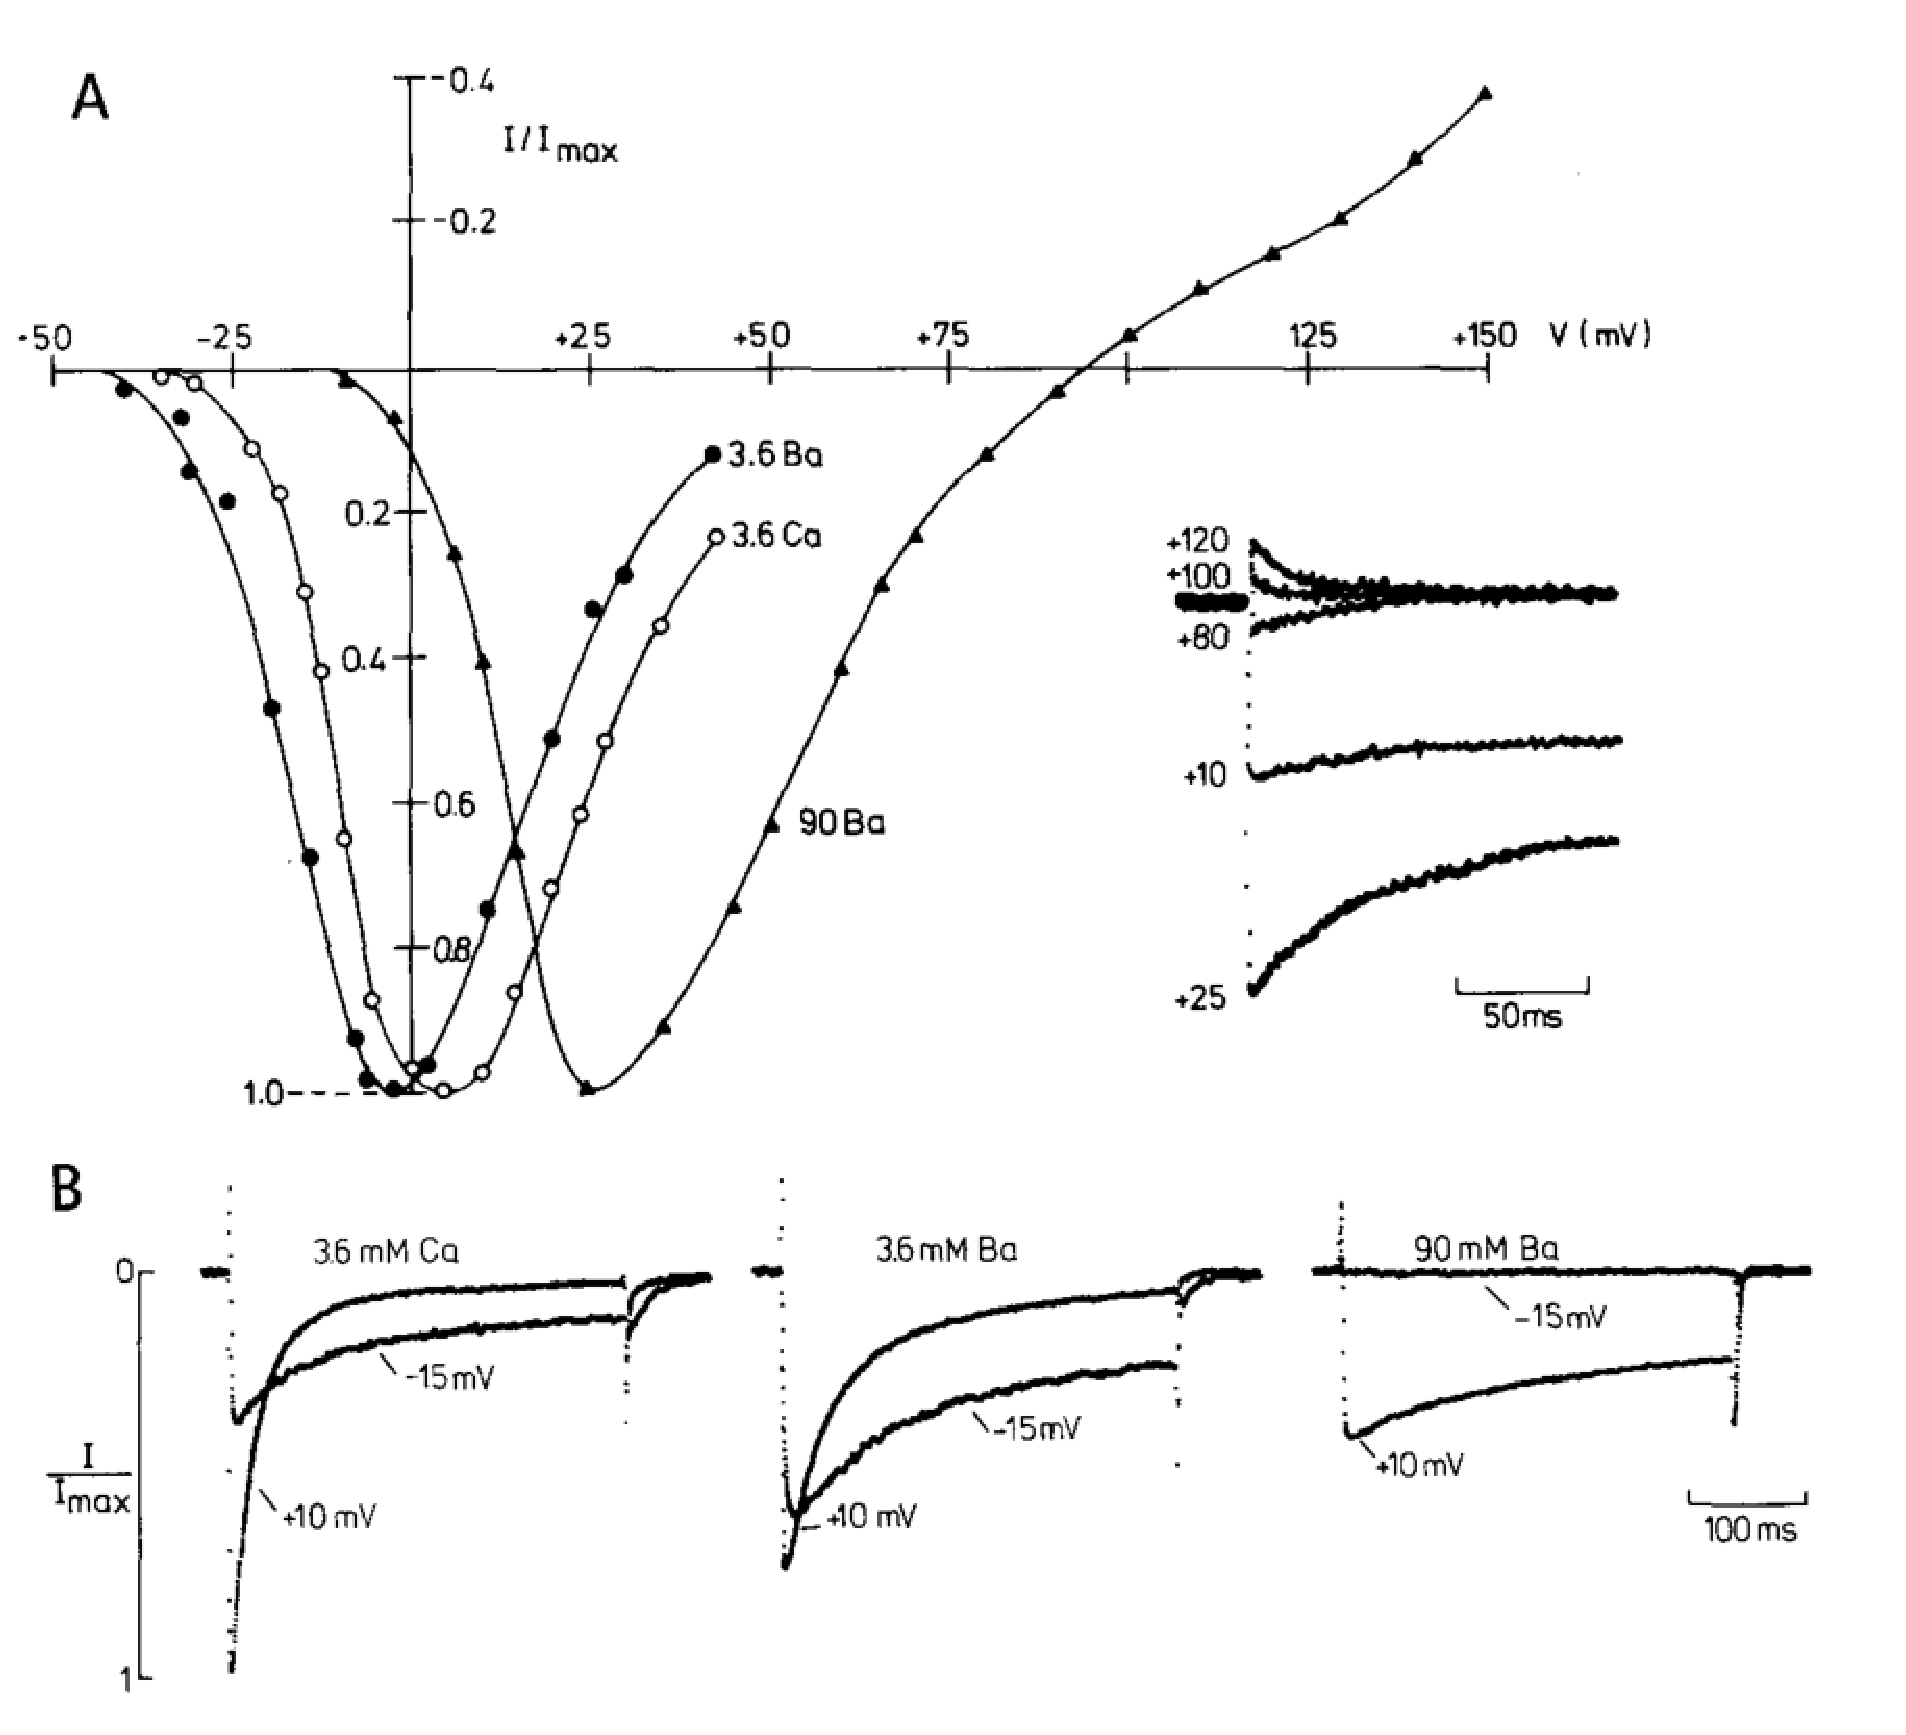
\includegraphics[height=5cm,
    angle=0]{./images/ICaL_McDonald1986.eps}; 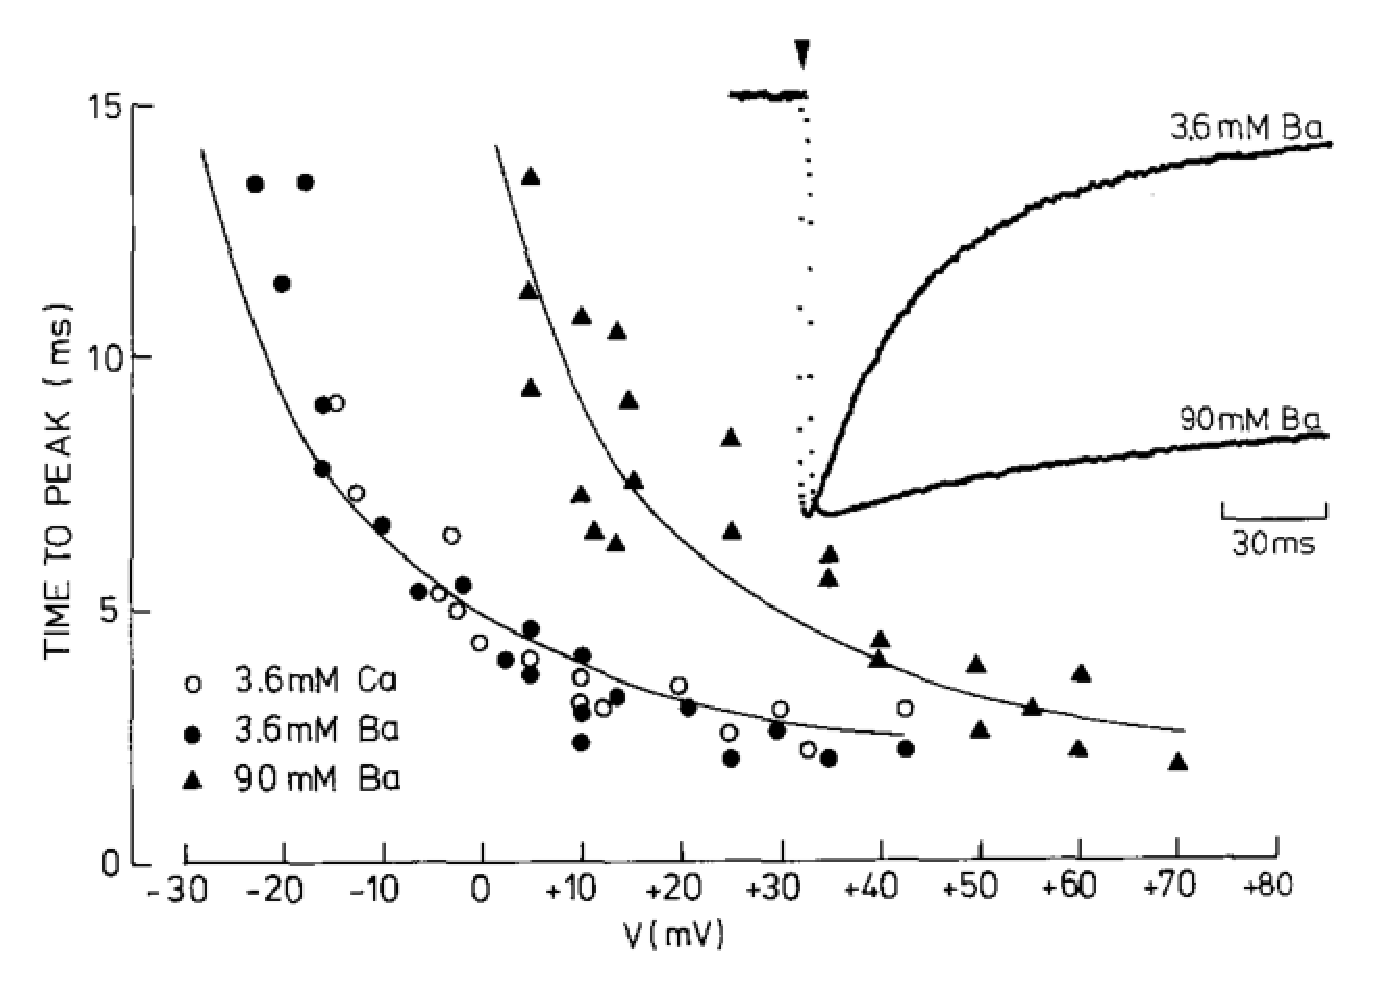
\includegraphics[height=5cm,
    angle=0]{./images/ICaL_time2peak_McDonald1986.eps}}
\caption{Using holding potential -50mV: (A) I-V  curve at 3.6mM $\Ca$
($\circ$); 3.6mM $\Ba$ (black circle), and 90mM $\Ba$ (filled triangle). (B)
currents recorded during 300ms pulse using pulse at -15mV or +10mV bathed in
3 different solutions conditions as described previously. (C) time to peak}
\label{fig:ICaL_McDonald1986}
\end{figure}



The activity of ion channels can be measured at molecular level since
1994 using patch-clamp \citep{mcdonald1994}. As opening of a single
LCC channel can trigger the $\Ca$ spark
(Chap.~\ref{chap:sparkology-study-ca}), to help modeling, it's
important to have an accurate native, unitary current measured at
physiological condition, i.e. in the absence of LCC agonist and
physiological concentration of calcium ions $[\Ca]_o$. 

Under physiological condition, the measured $I_\CaL$ is quite small (0.1-0.2 pA
with $[\Ca]_o =2$mM) \citep{church1996,guia1999,rubart1996,yue1990}. The
background noise is about 0.2-0.3 pA root-mean-square (RMS). So, it's hard to
distinguish the single channel current from noise. To increase signal-to-noise
ratio, there are 2 options:
\begin{enumerate}
  \item some tried to use a large
concentration of $[\Ca]_o$~\citep{imredy1994mcs}. However, it could potentially
change the kinetics of the channel. A
solution is to  use an alternate divalent ions, e.g. $\Ba$ (typically 70-110mM)
\citep{pietrobon1990,hirano1999} which yields higher unitary  current by
increasing the amplitude; yet it raised the problem that  the kinetics of the
channel, e.g. $\Ca$-dependent inactivation, is  bypassed. 

  \item prolong the opening of the channel usings some agonists
  (Sect.\ref{sec:DHPR_agonists}). A further complication is that the short unitary current ($\sim$ 1ms)
limits the amount of filtering that can be applied to remove the
background noise. To avoid this, a common strategy is to prolong the
opening of the channel using agonists like CGP28392, Bay K 8644, and
FPL64176 \citep{mcdonald1994,yue1990,imredy1994mcs, fan2000} to prolong the
duration of the channel opening. However, these agonist also change
$V_m$-dependent, amplitude and conductance of the channel as well,
e.g. in
heart \citep{kokubun1984,hess1986ccs,handrock1998,
  reuter1988,fan2000}, in smooth muscle \citep{caffrey1986}.
  \item 
\end{enumerate}

LCC is activated by membrane depolarization. The inactivation of LCC
during depolarization results from both
$V_m$-dependent \citep{hadley1987} and
$\Ca$-dependent \citep{lee1985icc}. At single channel level, the
$\Ca$-dependent inactivation shown a shift of gating from relatively
frequent, brief opening ({\bf mode 1}) to a lower open probability,
termed {\bf ``mode Ca''} \citep{imredy1994mcs}. There are also
evidences of {\bf mode 2} - a $\Ca$-independent increase in $I_\CaL$
(long-duration of opening, yet relatively frequent) at strong
depolarization
prepulse \citep{pietrobon1990, 
  josephson2002mgu}. \citep{josephson2002mcu}
shown that mode 2 not only have longer opening-duration, but also of
greater conductance than mode 1.

\begin{framed}
Agonists like Bay K 8644 can pharmacologically promote mode 2
long-openings,and can increases conductance by 25\% (from 12pS to 15pS
with 100mM $\Ba$) \citep{caffrey1986}.
\end{framed}

\subsubsection{Guia {\it et al.} (2001)}
\label{sec:guia-it-et}

\citep{guia2001} derived a method to measure $I_\CaL$ at physiological
condition, and determine concentration-dependent as well as
ion-species-dependent of $I_\CaL$ in native cardiac myocytes. The
result
\begin{enumerate}
\item single-channel conductance is 3pS with physiological
  concentration ($[\Ca]_o=2$mM); and maximum 5pS with high
  concentration. The value 3pS is closed with that in chick ciliary
  ganglion neuron (2.6pS) \citep{church1996}, and $\ca_{v2.2}$
  channels in chick dorsal root ganglion neurons
  (2.5pS) \citep{weber2009}.

  Using Barion \ce{Ba^2+}, maximal conductance is 15pS, i.e. 3-fold
  faster rate of passage through the pore.


\item
  \textcolor{red}{At 0mV, $[\Ca]_o=$2mM produces $I_\CaL=0.12$pA, and
    2mM of \ce{Ba^2+} yields 0.19pA unitary current}.
  The concentration of ions to produce the half-maximal current is not
  much difference between $\Ca$ and $\Ba$, i.e. $K_{m,\ca}=
  1.7\pm$0.3mM, and $K_{m,\Ba}=1.9\pm$0.4mM.
\end{enumerate}

To calculate the permeability for a single L-type $\Ca$ channel, we
apply eq.~\eqref{eq:1353} with $[\ca]_\myo=0.1\mu$M,
$[\ca]_o=2$mM=$2e3\mu$M, and $i_\dhpr=0.12$pA; at $V_m=-10$ mV
\begin{equation}
  \label{eq:1354}
  \begin{split}
    P_\dhpr &=  \frac{i_\dhpr}{z_\ca ^2 \frac{F}{RT/F}V_m
      \left[\frac{\exp\left(\frac{z_\ca V_m}{RT/F}\right)[\ca]_\myo-0.341[\ca]_o}{\exp\left(\frac{z_\ca V_m}{RT/F}\right)
          - 1} \right]} \\
    &=  \frac{0.12 [pA]}{4 \frac{9.6485d4[C/mol]}{26.7123387[mV]}(-10)[mV]
      \left[\frac{\exp\left(\frac{2*(-10)[mV]}{26.7123387[mV]}\right)0.1[\mu
          M]-0.341*(2e3)[\mu
          M]}{\exp\left(\frac{2*(-10)[mV]}{26.7123387[mV]}\right)
          - 1} \right]}
  \end{split}
\end{equation}

\subsubsection{Josephson et al. (2002)}
\label{sec:josephson-et-al}

Josephson et al. examined the role of prepulse (induce inactivation or
facilitation) and divalent ion (types and concentration) on (1) gating
of single LCC \citep{josephson2002mgu}, and the
conductance \citep{josephson2002mcu} of single LCC current. The
divalent ions to tested were $\Ca$ at nearly physiological
concentration ($[\Ca]_o=$5mM), and a range of concentration of $\Ba$
ions, both in the absence of any agonists.

\subsubsection{Recording techniques}
\label{sec:recording-techniques}

The technique to record is the same as \citep{guia2001}
(Sect.~\ref{sec:guia-it-et}). Data is recorded at room temperature
(22.5-23.5$^\circ$C). Currents are amplified using Axopatch 200B patch
clamp (Axon Instruments Co.) and recorded to computer using PClamp
software (v.6 and v.8) via Digidata 1200A acquisition system. Data are
then Gaussian filtered 2kHz \citep{sakmann1983} and digitized at 10kHz
sampling rate.

To study the effect of prepulse, A {\bf double voltage-step protocol}
was used, i.e. each 100 ms
prepulse\footnote{\url{http://en.wikipedia.org/wiki/Depolarizing_pre-pulse}},
using potential from -50mV to +130mV (with increment 20mV, i.e. 10
steps) was immediately followed by 300-400ms test voltage step -10mV
or 0mV.  The rate to apply the 10-step protocol above is 0.5Hz (to
allow complete recovery between runs), from a holding potential
$V_m=-50$mV.  The 10-step protocol was repeated 100-200 times, or
until the channel rundown was observed.

\begin{framed}
  The 100ms prepulse was chosen because it doesn't produce complete
  $V_m$-dependent inactivation. This allows a relative ion
  concentration-dependent effects on inactivation and facilitation. 
\end{framed}

Data file, each contain the episodes recorded at a given prepulse
potential. Leak currents and capacity currents were subtracted out by
subtracting the average of episodes.
\begin{itemize}
\item {\it Event detection}: Single LCC opening/closing was identified
  based on 50\% amplitude threshold (set constant for each experiment)
  using Fetchan 6.0/PClamp.
\item The rise time of the recording system is 0.166ms at 2kHz, so any
  events shorter than 2ms are not included in the kinetic analysis.
The fraction of maximum amplitude attained by an event, $A_\max/A_o$
is given \citep{colquhoun1995fsa}
\begin{equation}
  \label{eq:1422}
  A_\max/A_o=\erf(0.886.w/\tau_r)
\end{equation}
with $\erf(\cdot)$ is error function, $w$ is the duration of the
event, $\tau_r$ is the rise time of the filter.  So, channel events of
$w=0.5$ms attain 99\% of their amplitude after filtering. By limiting
the analysis to opening of $w=0.5$ms and higher, this eliminate the
possibility that full amplitude of brief (mode 1) opening were
significantly modified due to the filtering process.

\item number of active LCC in the patch (N) was estimated by the
  maximum number of overlapping currents recorded upon repolarization
  following a prepulse of +130mV (to get maximal activation, and
  synchronization of mode 2 openings). The probability for openings is
  then calculated as the sum of all open time detected divided by the
  total episode time averaged over the test voltage step.
\end{itemize}

The data analysis (probability of opening, open-time distribution with
their exponential fit, amplitude distribution with the Gaussian fit,
and scatter-plot of amplitude) were done using a modified version of
pSTAT (PClamp, Axon Instruments). For significant testings, they used
ANOVA, Dunnett's method. or Student's paired t-test. 

\subsubsection{Results}
\label{sec:results-1}

They decided to test the Voltage-dependent effects of conditioning
prepulse, using different level of $\Ba$ and $\Ca$,
Fig.~\ref{fig:josephson2002}. Using 105mM $\Ba$, a test voltage
(-10mV) for 400ms from a holding potential -50mV shown frequent LCC
opening and were nearly time-invariant during the test pulse. However,
combining the test pulse with +10mV prepulse for 100ms, the channel
opening during the test step was less frequent, i.e. partial
inactivation. The interesting part is that using a much higher
prepulse (+110mV), the channels increased the activity (mode 2); or
the large positive prepulse induced facilitation of channel activity.

Using 5mM $\Ba$ (test step is now 300ms), a similar, but slightly
different, pattern is observed.

Using 5mM $\Ca$ (protocol like 105mM $\Ba$), the role of prepulse is
similar, yet the subsequent frequency of re-opening was reduced, as
compared to $\Ba$. \textcolor{red}{In summary, depending upon the
  value, prepulse show either inactivation or facilitation of $\Ca$
  channel activity}.

\begin{figure}[hbt]
  \centerline{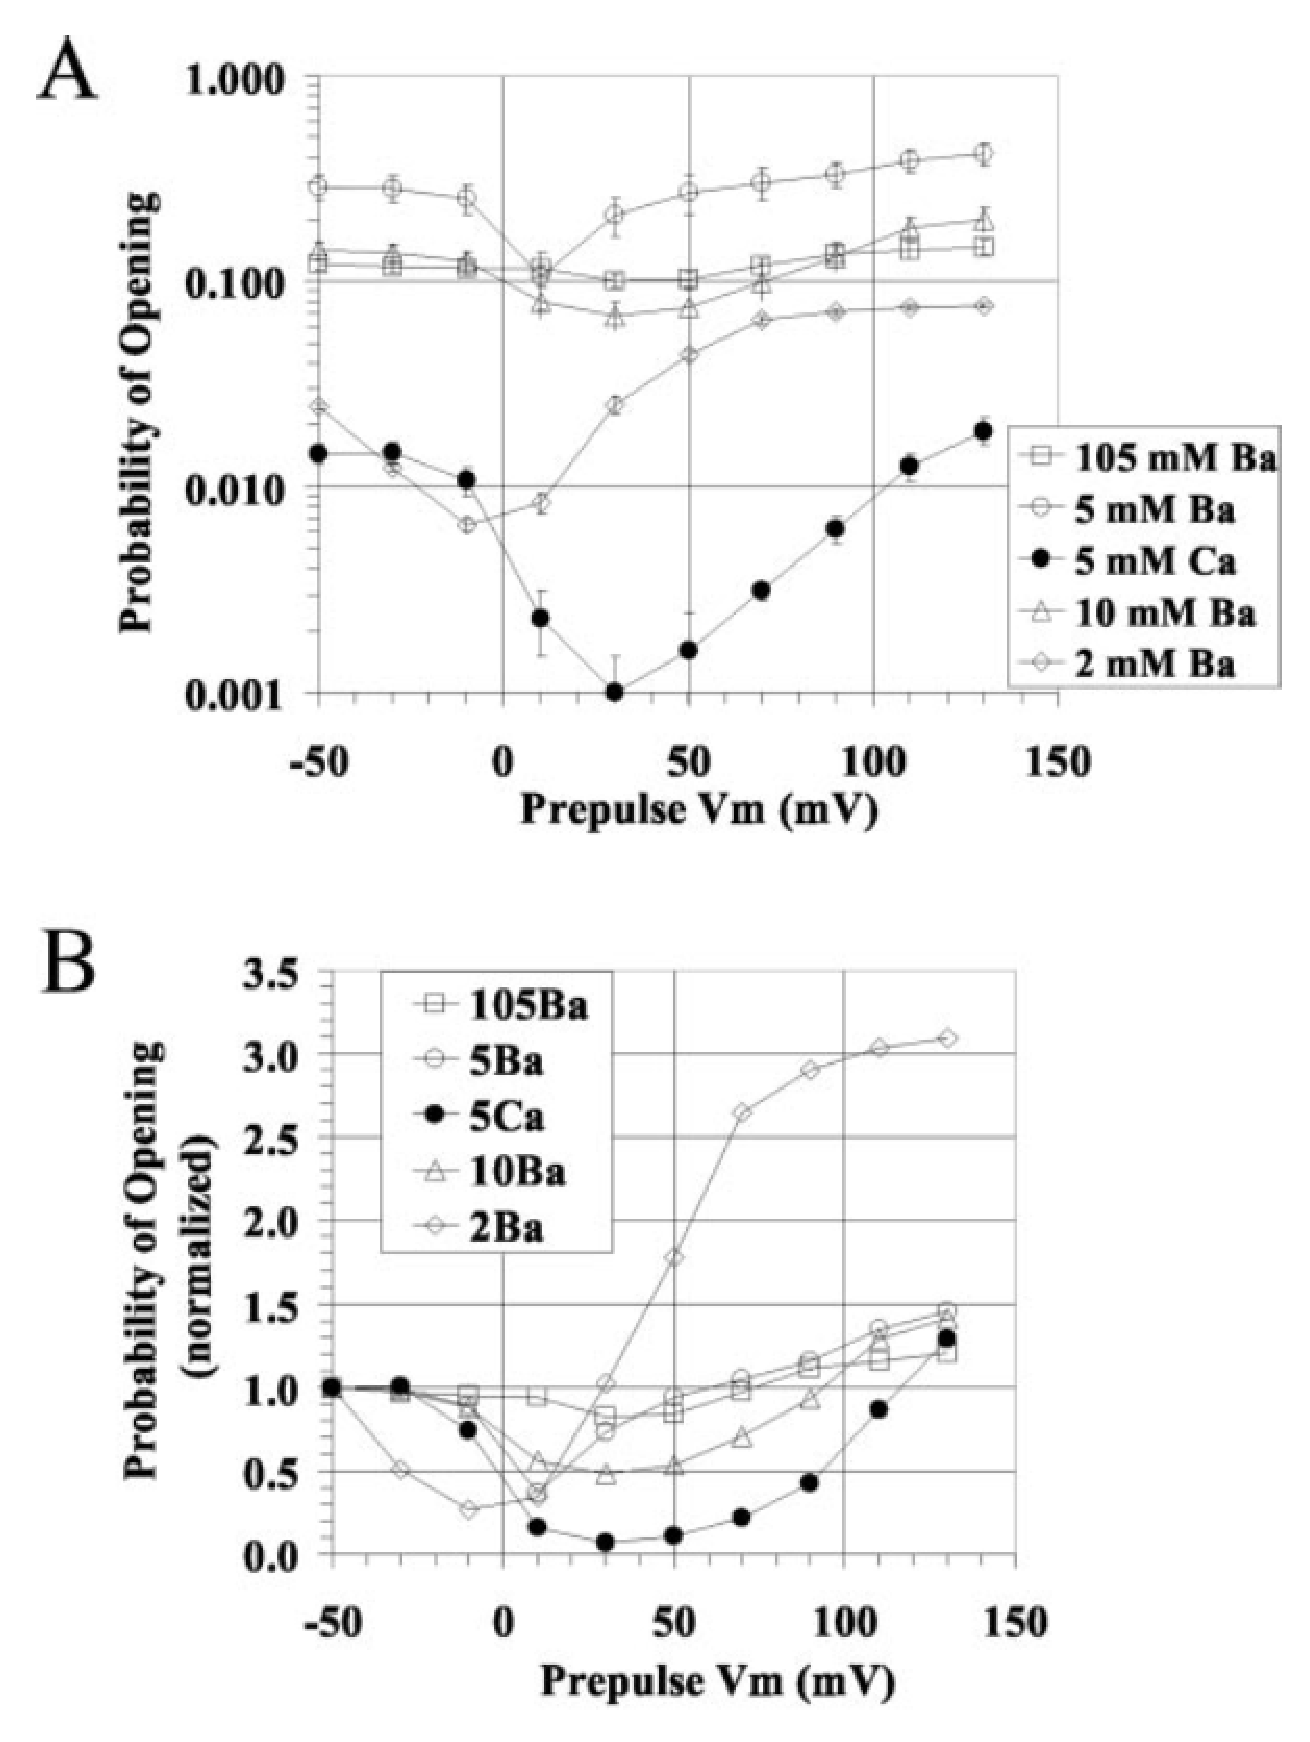
\includegraphics[height=6cm,
    angle=0]{./images/josephson_2002.eps}}
  \caption{Effect of 100ms prepulse on $P_o$ of LCC during the test
    step. (A) The plot is logarithmically or averaged probability of
    opening $p_\avg$ (averaged over multiple test step for a given
    prepulse). (B) data in A were normalized to their values at -50mV
    (without a prepulse). Values $<1.0$ represent inactivation, values
    $>1.0$ represent facilitation of single channel currents.}
  \label{fig:josephson2002}
\end{figure}

As shown in Fig.~\ref{fig:josephson2002}(A), $p_\avg$ during the test
step (test pulse) decreased with increasing prepulse, and reached a
minimum at
\begin{itemize}
\item -10mV for 2mM $\Ba$
\item +10mV for 5mM $\Ba$
\item +30mV for 10mM $\Ba$
\item +30 to +50mV for 105mM $\Ba$
\item +30mV for 5mM $\Ca$
\end{itemize}
If the prepulse is more positive, $p_\avg$ returned to its initial
value; and even higher above the value without the prepulse if the
prepulse is of greater positive. This single channel current is
similar to whole-cell level $\Ca$ channel current. 

To obtained a precise comparison, the data are normalized to
$\overline{p}_\avg$ obtained at -50mV holding potential,
Fig.~\ref{fig:josephson2002}(B).
\textcolor{red}{The (maximal extent) degree of prepulsed-induced
  inactivation decreased with increasing $\Ba$ concentration or we can
  say the degree of facilitation decreases with increasing $\Ba$
  concentration},
i.e. the maximal extent of inactivation of $p_\avg$ is: 74\% (2mM
$\Ba$), 63\% (5mM $\Ba$), 52\% (10mM $\Ba$), and 18\% (105mM
$\Ba$). The maximal extent of inactivation of $p_\avg$ was greatest
with 5mM $\Ca$ (94\%). At high positive prepulse, +130mV, the
facilitation increase (compared to the $p_\avg$ with no prepulse) 36\%
(105mM $\Ba$), 46\% (5mM $\Ba$), 392\% (5mM $\Ba$), and 258\% (5mM
$\Ca$).

% The shifting (to left or right) in U-shape inactivation/facilitation
% curve is caused by the type and concentration of divalent ions,
% Fig.~\ref{fig:josephson2002}.
The threshold for $\Ca$ channel activation was:
\begin{itemize}
\item -40mV to -30mV for 2mM $\Ba$
\item -30mV to -20mV for 5mM $\Ba$
\item -10mV to 0mV for 105mM $\Ba$
\item -30mV to -20mV for 5mM $\Ca$
\end{itemize}
$P_o$ for $\Ca$ channel using nearly physiological concentration
$[\Ca]_o=5$mM is $\sim 10$-fold lower than that recorded with
$\Ba$. This is further dramatically reduced with a +10mV prepulse,
i.e. most episodes displaying no channel openings (Fig.3 in paper). 

The previous paragraphs discuss the effect on probability of opening.
\textcolor{red}{How about prepulse effect on the opening time
  $\tau$?}.
They assume the opening times are classified into 3 classes: fast time
constant $\tau_1$, medium time constant $\tau_2$, and slow time
constant $\tau_3$. So, the distribution of open-time is the sum of 3
exponential components (which showed a better fit than the sum of
2\footnote{they compared to choose the better one using ``F''-value
  (goodness-of-fit criteria) calculated form the sum of squared errors
  for the two models in pSTAT}).
The result (Table 1 in the paper) is given in
Fig.~\ref{fig:josephson2002-tau}.

\begin{figure}[hbt]
  \centerline{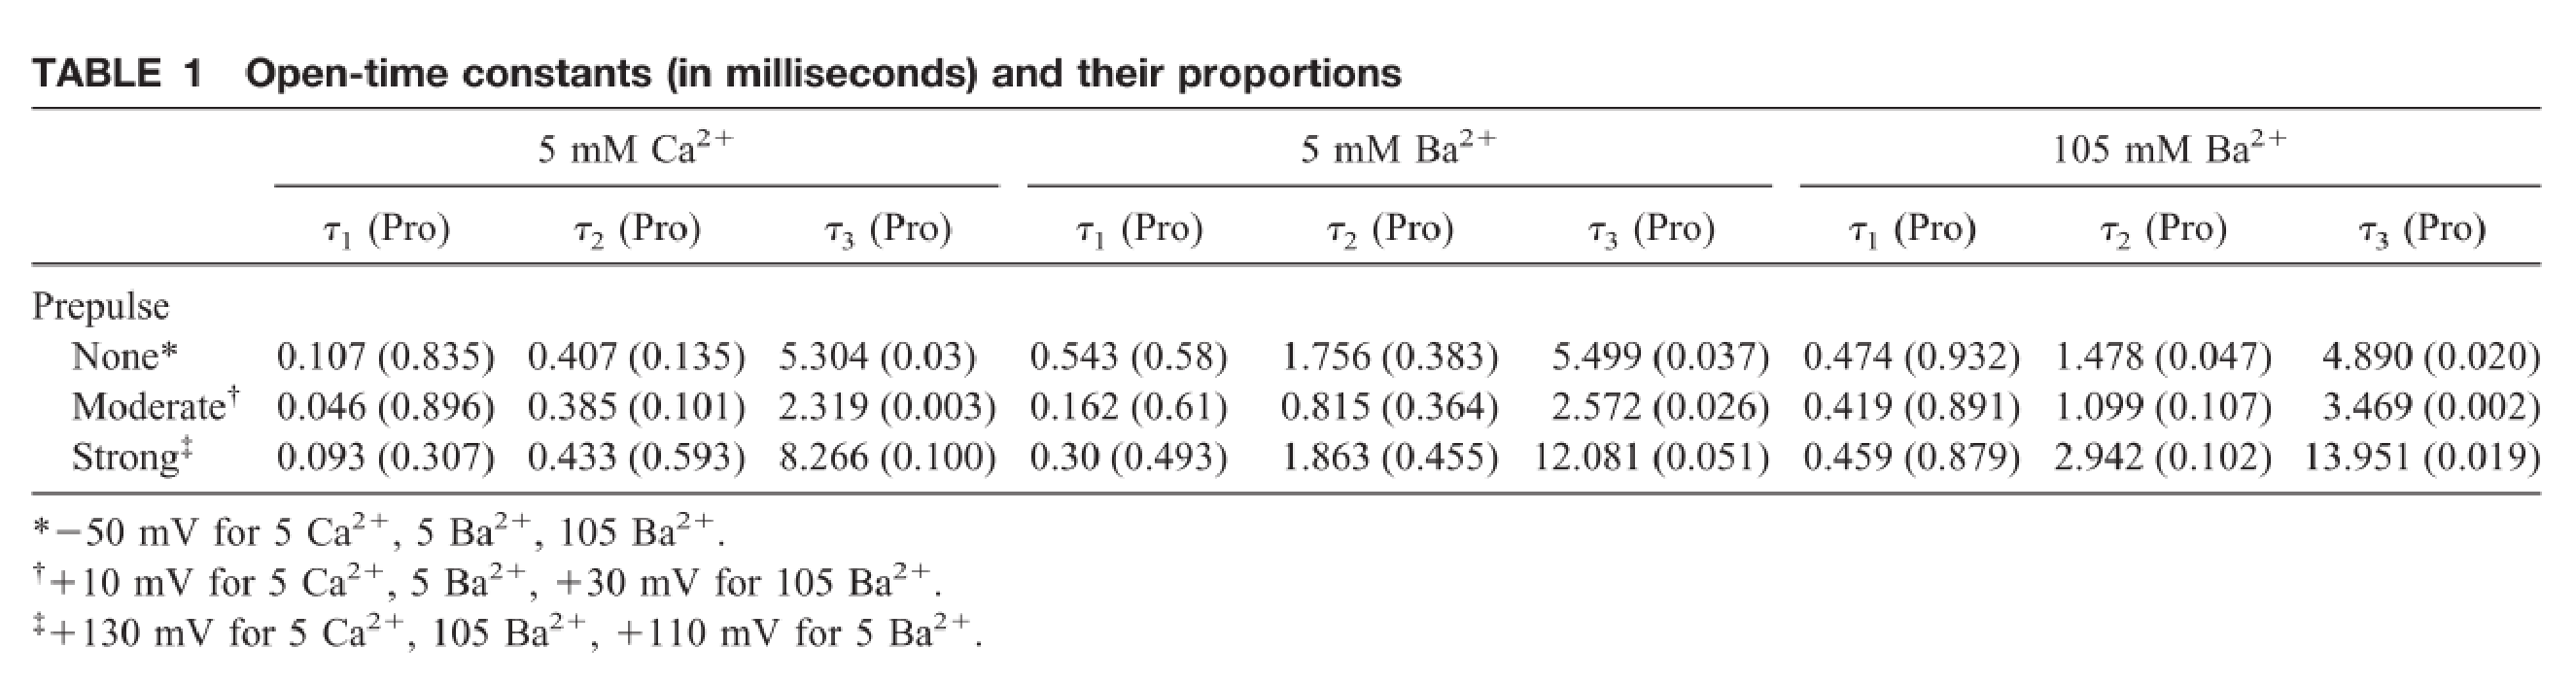
\includegraphics[height=4cm,
    angle=0]{./images/josephson_2002-tau.eps}}
  \caption{Table 1. open time constant (ms) and their proportions
    (\%)}
\label{fig:josephson2002-tau}
\end{figure}


\textcolor{red}{How about the role of prepulse and ion-species on
  conductance and current amplitude?}.
For current amplitude, using the sum of 2 Gaussian distributions to
fit the amplitude distributions, the mean amplitudes are (with 105mM
$\Ba$)
\begin{itemize}
\item absence of prepulse: $-1.13\pm0.1$pA (14\%) and $-0.89\pm0.2$pA
  (86\%)
\item with prepulse +110mV and test pulse 0mV: $-1.17\pm0.074$pA
  (32\%) and $-0.92\pm0.057$pA (68\%)
\end{itemize}
Clearly, there's an increase $\sim 27\%$ of average amplitude in long
duration (mode 2). Fitting with 2 Gaussian distributions for the cases
of 5mM $\Ba$ and 5mM $\Ca$ (both with prepulse +100mV, the results
are:
\begin{itemize}
\item 5mM $\Ba$: $0.56\pm0.08$ pA (21\%) and $0.42\pm0.08$ pA (79\%),
\item 5mM $\Ca$: $0.30\pm0.1$ pA (39\%) and $0.25\pm0.1$ pA (61\%)
\end{itemize}

\textcolor{red}{The relation between current amplitude and duration of
  channel opening during test pulse were studied as well}.
Using scatter plot, brief events distribute symmetrical about the
average amplitude. In mode 2, however, the current are higher than
average amplitude \citep{josephson2002mcu}.  The opening were
classified into 2 groups: short and long.  The cutoff for the shorter
events was $<3.5$ ms for 105mM $\Ba$ and for 5mM $\Ba$, and $<2.0$ ms
for 5mM $\Ca$. As pointed out above, the events with $<.5$ms are
excluded from analysis.
\begin{itemize}
\item 105mM $\Ba$: prepulse-induced short opening is $-0.91\pm0.22$pA,
  and long-duration (prepulse: +110mV, step 0mV) has $-1.16\pm0.13$pA,
  which is 27\% larger in magnitude than short opening.
\item 5mM $\Ba$: ... has $-0.39\pm0.03$pA, and ... $-0.50\pm0.06$pA
  which is 28\% increase.

\item 5mM $\Ca$: ... (test -10mV) has $-0.24\pm0.06$pA,
  ... $-0.30\pm0.07$pA, which is 25\% increase.
\end{itemize}

For conductance, the slope conductance (measuring tail current
(i.e. near the end of the test pulse and remain opening) in the case
of $\Ba$, and during voltage step for $\Ca$ (as tail current is rare))
\begin{itemize}
\item 105mM $\Ba$: $25.7\pm1.2$pS for long-opening and $14.5\pm0.5$pS
  for all openings.
\item 5mM $\Ba$: $18.2\pm.6$pS... and $10.8\pm0.4$pS ...
\item 5mM $\Ca$: $6.1\pm0.3$pS and $3.6\pm0.2$pS for all openings
\end{itemize}


In summary, high positive prepulse shown a 10- to 100x increase in
mean open time $\tau$, and 70\% increase in conductance. The frequency
of mode 2, in the absence of prepulse or agonists, depends on many
factors, e.g. species, endogenous intracellular levels of cAMP... In
mode 2, they hypothesized that
\textcolor{green}{the channel may loss divalent selectivity, allowing
  monovalent to go through. This loss may be facilitated by high
  voltage prepulse}. This needs to be tested. 


With a physiological $\Ca$ concentration $[\Ca]_o=1.8$mM, the
$V_m$-dependence for activation would be shifted to the left
(i.e. less positive). The deactivation in mode 2 is relatively slow
compared to mode 1 (especially at depolarized potential), mode 2
openings would be continuing during the repolarization process. This
may explain for the late $\Ca$ influx during repolarization.


\subsubsection{Josephson et al. (2010)}
\label{sec:josephson-et-al-1}

The scarcity of unitary LCC current at physiological range was due to
technical difficulty. Even though, the previous research
(Sect.~\ref{sec:josephson-et-al}) has made an effort to use nearly
physiological $[\Ca]_o=5$mM, Josephson et a. made a progress to use
physiological value $[\Ca]_o=$2mM to study $V_m$-dependent gating
kinetics on peak $P_o$ and dwell-time \citep{josephson2010pgp}, and to
study $\Ca$-dependent gating kinetics \citep{josephson2010cdc}, both
in the absence of LC agonists.

\subsubsection{Recoding techniques}
\label{sec:recoding-techniques}

Similar to Sect.~\ref{sec:recording-techniques}. One change: data
analysis and non-linear curve fitting were performed using Origin v7.5
(OriginLab Corp, USA).

\subsubsection{Results}
\label{sec:results-2}

The peak opening probability for single LCC channel is calculated from
eq.~\eqref{eq:1423} with $i_\ca$ is from~\citep{guia2001}
(Sect.~\ref{sec:guia-it-et}). $P_o$vs.$V_m$ was fitted using Boltzmann
distribution with maximum value 0.3, midpoint is -12mV, and slope
factor 8.5. The slope can be used to calculate the number of gating
charges of channel activation $z_g$
\begin{equation}
  \label{eq:1424}
  z_g = k(RT/F)
\end{equation}
with $RT/F=25$mV, which give 3 electric charges are transferred across
the membrane electric field during the channel activation. The average
number of ions entering the cell through a single opening of
individual LCC is 300-400 ions, remains relatively constants over the
range of potential from -30mV to 0mV.

\begin{figure}[hbt]
  \centerline{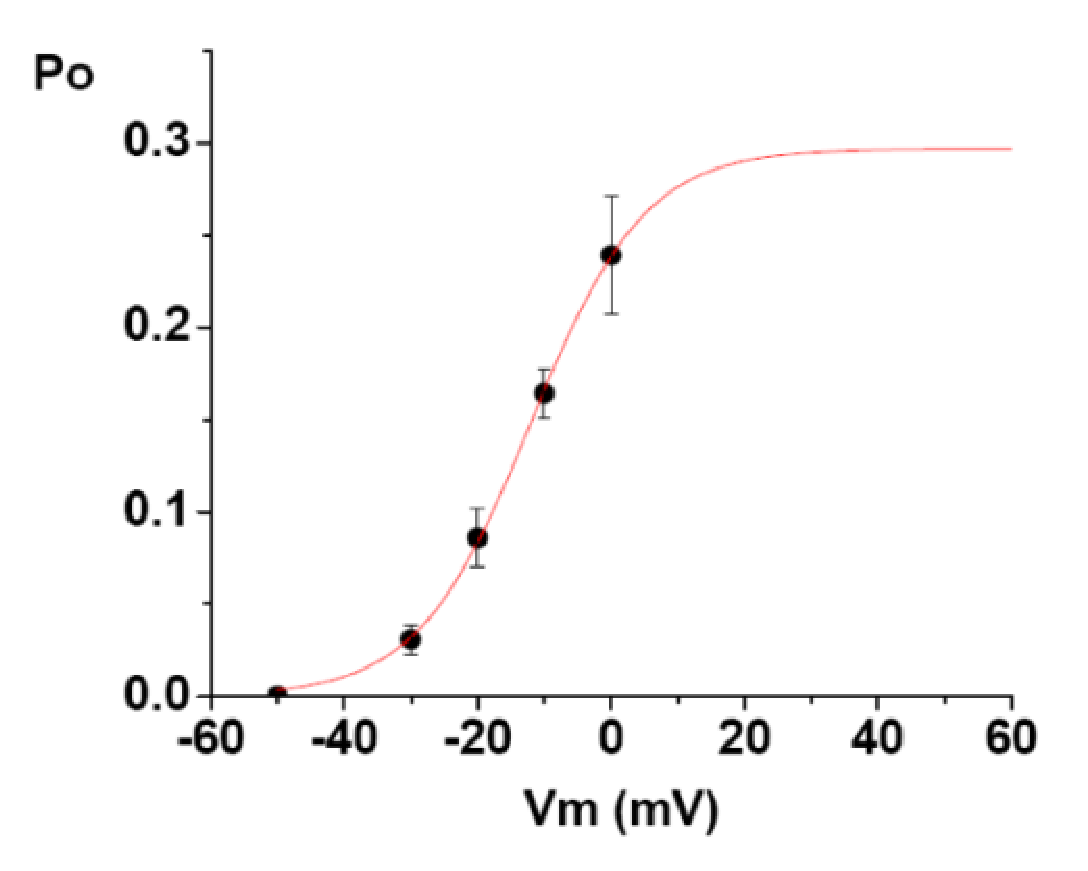
\includegraphics[height=5cm,
    angle=0]{./images/josephson_2010_Po.eps}}
\caption{$P_o$ vs. $V_m$ shown a sigmoidal function, best fitted with
  a Boltzmann equation}
\label{fig:josephson_2010_Po}
\end{figure}

As shown in Fig.~\ref{fig:josephson_2010_Po}, the peak $P_o=0.3$ at
$V_m=+30$mV. Using computational model, \citep{greenstein2002}
estimated $P_o=0.05-0.15$. From other experimental
studies,~\citep{herzig1993,handrock1998} used 70mM $\Ba$ and
\citep{rose1992} used 10mM $\Ca$, \citep{rose1992} yielded peak
$P_o=0.03$ which is an order of magnitude lower than the present
finding. \textcolor{red}{So, $P_o$ need to be investigated further to
  have a more accuracy value}. 

The dwell open time ($\sim 0.2$ms) is brief and has been assumed to be
$V_m$-independent. However, the present study find an increase in
dwell-time with depolarization, Fig.~\ref{fig:josephson_2010_tau}. So,
this MOT increase counterbalance the decrease in unitary LCC amplitude
with depolarization, so that average $\Ca$ influx to be relatively
constant across a range of potential. 

\begin{figure}[hbt]
  \centerline{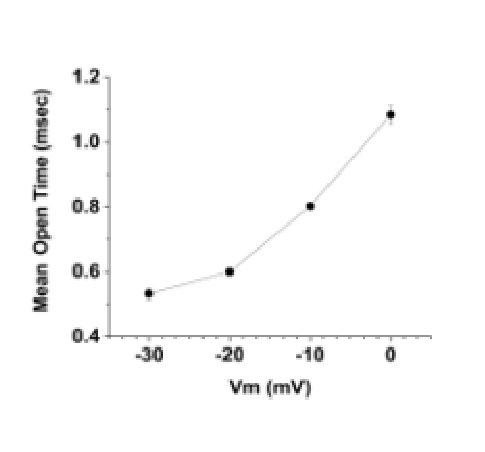
\includegraphics[height=5cm,
    angle=0]{./images/josephson_2010_tau.eps}}
\caption{Mean open time (MOT), recorded using 2mM $\Ca$ measured at
  100ms test step}
\label{fig:josephson_2010_tau}
\end{figure}


%\section{Voltage-gated calcium channels (VGCC)}
%\label{sec:VGCC}
\chapter{Store-operated calcium channels (SOC; on plasma membrane)}
%\section{Store-operated calcium channels (SOC; on plasma membrane)}
\label{sec:store-operated-calcium-channel}
\label{sec:SOC}
\label{sec:capacitative-calcium-entry}
% \section{Capacitative calcium entry}
% \label{sec:capacitative-calcium-entry}


The concept {\bf capacitative model} for store-operated calcium entry
(Sect.\ref{sec:store-operated-calcium-entry}) lead to a proposal whereby the
activation of Ca2+ influx occurred secondarily to the depletion of the
endoplasmic reticulum Ca2+ pool (Putney, 1986),
Fig.\ref{fig:PLC-activated-Ca2+-influx}.
\begin{itemize}
  \item  In 1992: the first report by Hoth and Penner (Hoth \& Penner, 1992) of
  a membrane current activated by Ca2+ store depletion in mast cell.

This current has been described in an earlier report from another laboratory
(Lewis \& Cahalan, 1989) for human leukemic T cells but it was not recognized as
such - Sect.\ref{sec:calcium-oscill-waves}.

Hoth and Penner (Hoth \& Penner, 1992) called the current calcium
release-activated calcium current or Icrac (Sect.\ref{sec:Icrac}).

  \item 
\end{itemize}


\begin{figure}[hbt]
  \centerline{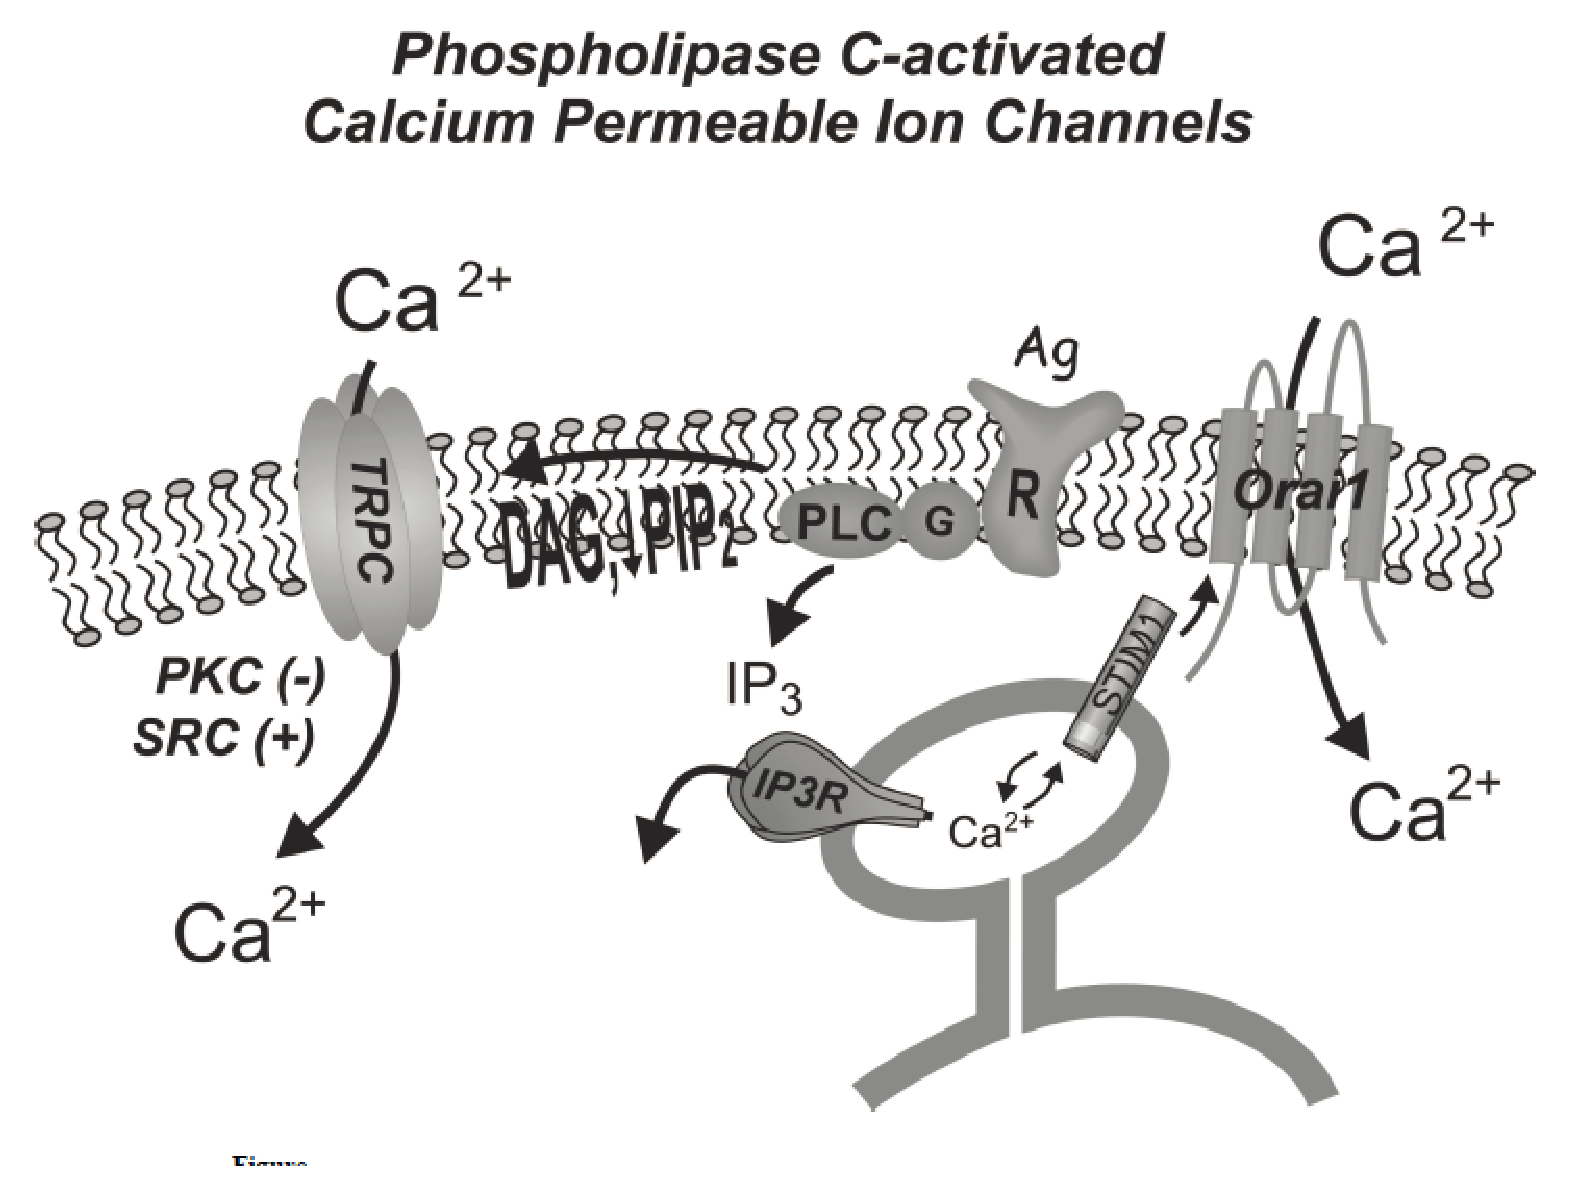
\includegraphics[height=4cm,
    angle=0]{./images/PLC-activated-Ca2+-influx.eps}}
  \caption{Agonist (Ag)-activated GPCR receptor links to PLC activation, which
  cleave PIP2 into DAG and IP3. IP3 trigger $\Ca$ release from ER via IP3R.
  The drop in ER Ca2+ activates a Ca2+ sensor, STIM1 (Sect.\ref{sec:STIM1}),
  that redistributes within the endoplasmic reticulum to sites where it can
  interact with Orai1 (Sect.\ref{sec:Orai}). Another class of less selective,
  Ca2+-permeable channels, the
TRPCs (Sect.\ref{sec:TRPC}), are activated by PLC, most likely by changes in
membrane composition of DAG and PIP2. Not shown in this figure is a presumed complex interaction between the
pathways involving the translocation of TRPC channels to the membrane in response to
Ca2+ entering through Orai1 channels (see (Cheng et al., 2011)).}
  \label{fig:PLC-activated-Ca2+-influx}
\end{figure}


Its other names: CRAC = calcium-release activated calcium channels (or
currents); SOC channels. As the activation of CRAC is due to the change in
internal calcium store - ER; CRAC is also known as {\bf store-operated calcium
chananels} (SOC channels).

% SOC channels refer to calcium-pereable channels on plasma-membrane that are
% activated upon the depletion of $[\Ca]_\ER$, via the intermediate of STIM1
% protein on the ER membrane. It is known as ``store-operated" or the
% "capacitative" mechanism.

The loading status of the endoplasmic reticulum regulates plasma membrane Ca2+
influx was initially called {\bf capacitative calcium entry} because of the
analogy with electrical circuitry wherein a resistance (plasma membrane) and
capacitance (Ca2+ store) in series mutually regulate one another.
However, today perhaps the more popular term is {\bf store-operated calcium
entry} occurring through {\bf store-operated calcium channels}
\citep{putney1999} (Putney - Tomita, 2012).



Capacitative calcium entry appears to also be a major means of signal
transduction in electrically {\it non-excitable cells}, e.g. lymphocytes.


\begin{mdframed}

The question is {\bf how $[\Ca]_\ER$ deplete in the first place?} The answer can
be GPCR (Sect.\ref{sec:GPCR-PLC-IP3-DAG-pathway}) activating PLC which produces
IP3 (Sect.\ref{sec:ip3-pathways}) and IP3 in turn mediates the discharge of Ca2+
from intracellular stores (components of the endoplasmic reticulum).

Putney (1986) proposed that the activation of a receptor (GPCR) which was linked
to the formation of IP3 might trigger the entry of $\Ca$ via a biphasic process
in non-excitable cell, e.g. rat parotid acinar cell \citep{putney1986,
takemura1989}.
% Takemura H, Putney JW. Capacitative calcium entry in parotid acinar cells. Biochem J. 1989;
% 258:409-412..

\end{mdframed}

CRAC proteins typically have between 4 and 6 transmembrane $\alpha$-helical
spanners (TMSs); with 4TM channels is the loss of 2TMs from 6TM channels.
Almost all CRAC homologues are about 250 residues long, but some are up to 100
residues longer.


\section{Orai: ORAI1, ORAI2}
\label{sec:Orai}
\label{sec:ORAI1}

The plasma membrane protein "Orai" (ORAI1 and ORAI2 in humans) forms the pore of
a type of calcium-permeable channels - {\bf calcium-release activated calcium
influx (CRAC) channel}; without needing membrane depolarization. There are three
genes encoded for the channel: Orai1, Orai2, and Orai3.

\begin{itemize}
  \item  ORAI1 open with it interacts with the STIM1 protein
  (Sect.\ref{sec:STIM1}).
\end{itemize} 



\section{TRP (Transient Receptor Potential) channels}
\label{chap:TRP}
\label{chap:TRP-family}

Review: \citep{ramsey2006}

Transient Receptor Potential (TRP) channels were discovered while analyzing
visual mutants in {\it Drosophila}. The photoreceptor, i.e. protein encoded by
the transient receptor potential (trp) gene, responds to light and activate a
{\it Ca(2+) permeable cation channel} that is regulated by PLC -
(Sect.\ref{sec:TRP-regulator}).



{\it trp} is a Drosophila photoreceptor mutant incapable of maintaining a
sustained receptor potential in response to photostimulation.
Because insect photoreceptors utilize a phospholipase C signaling system, this
phenotype suggested to Hardie and Minke that trp might encode a component of the
calcium entry pathway.

The sequence of TRP suggested a homology to the sequence of mammalian
voltage-dependent calcium channels. The idea that TRP could function as a
capacitative calcium entry channel was first examined by Schilling and
coworkers (Sect. \ref{sec:TRP-classification}).

Mammalian TRP-related genes were initially cloned in two
different laboratories

\section{TRPC channels (canonical)}
%\label{sec:TRPC}
%\section{TRPC}
\label{sec:TRPC}

TRPC is the mammalian TRP homologs (Sect.\ref{sec:TRP-classification}) TRPC all
appear to encode Ca2+ permeable, but relatively non-selective cation channels
with properties clearly distinct from Icrac (Sect.\ref{sec:CRAC} (Trebak et al.,
2003b;Beech et al., 2004;Venkatachalam \& Montell, 2007)..

There are 7 different genes: TRPC1, TRPC2, TRPC3, TRPC4, TRPC5, TRPC6, TRPC7
\begin{itemize}
  \item in general: TRPC can be activated by PKC, with some activated by DAG.
  
  \item TRPC1 also activated by stretching of the membrane
  
  \item TRPC3 regulate RyR1 (Sect.\ref{sec:RyR1})

Knockout of TRPC3 in primary skeletal myotubes demonstrates impaired RyR1
excitation-contraction (EC) coupling gain and SR Ca2+ release with intact SR
store Ca2+ levels.
  
  \item TRPC5 also activated by extracellular reduced thioredoxin
  
\end{itemize}

It has long been suggested that TRPC are store-operated channels (SOC) which
open due to the depletion of intracellular calcium stores.
However, two other proteins, stromal interaction molecules (STIMs) and the
Orais, have more recently been implicated in this process (Sect.\ref{sec:SOC}).
TRPC is a class of less selective, Ca2+-permeable channels, and is activated by
PLC (Sect.\ref{sec:PLC-Calcium}), most likely by changes in membrane composition
of DAG and PIP2.

A third possible scenario is TRPC1 and STIM1 cossemble to underlying SOCE
(Sect.\ref{sec:SOCE}). Some TRPC channels are inhibited by protein kinase C
and/or require the tyrosine kinase, src. 

In {\bf mammalian brain}: the predominant TRPC channels are the TRPC1, TRPC4 and
TRPC5 and they are densely expressed in corticolimbic brain regions, like the
hippocampus, prefrontal cortex and lateral septum.
\begin{itemize}
  \item TRPC 1,4,5 are activated by metabotropic glutamate receptor group 1
  (Sect.\ref{sec:mGluR}) agonist DHPG

  \item TRPC6 has been implicated in late Alzheimer's diseases
\end{itemize}

In {\bf heart}:
\begin{itemize}
  \item TRPC1 channels are found on cardiomyocytes, smooth muscle, and
  endothelial cells
  
  \item TRPC1 activated by receptors coupled to PLC (Sect.\ref{sec:PLC}), 
  mechanical stimulation, and depletion of intracellular $\Ca$ stores.
  
  \item TRPC1 channels mediate smooth muscle proliferation, linking to
  myocardial hypertrophy.
  
  \item TRPC3 and TRPC6 are activated by PLC stimulation and DAG production


  
  \item TRPC3 is upregulated in the atria of patients with atrial fibrillation
  (AF); TRPC3 regulates angiotensin II-induced cardiac hypertrophy which
  contributes to the formation of fibroblasts which can manifest into AF.

  \item upregulation of TRPC1, TRPC3, and TRPC6 genes found in heart diseases
  (e.g. fibroblast, cardiovascular hypertrophy)
  
MECHANISM: through activation of calcineurin pathway
(Sect.\ref{sec:calcineurin}) and the downstream transcription factor NFAT
(nuclear-factor of activated T-cell).
\end{itemize}

\section{TRPV channels (vanilloid)}
\label{sec:TRPV-channel}

TRPV channels belong to TRP family (Sect.\ref{sec:TRP-classification}).
All TRPVs are highly calcium selective.
 		
\section{TRPV1 channels}
\label{sec:TRPV1-channel}

To date, the most studied member of the TRP family is the TRPV1 

\section{TRPV4 channels}
\label{sec:TRPV4-channel}

TRPV4 is a member of TRPC channel (Sect.\ref{sec:TRPV-channel}).
The channel is activated by osmotic, mechanical and chemical cues. It also
responds to thermal changes (warmth). 


\section{ -- Structure and Classification}
\label{sec:TRP-structure}

Transient receptor potential channels (TRP) is a 6-transmembrane (6-TM)
cation-permeable channels. 

Like other 6-TM channels (example: Sect.\ref{sec:6TM/P}), TRPs probably form a
tetrameric quaternary structure, with each subunit contributes to a shared
selectivity filter and ion-conducting pore similar to that seen in $\K$
channels. The subunits are coupled via allosteric interaction to control {\it
one or more gates}, yet the location of the gate(s) in TRP channels is not
known.


\section{ -- Classification}
\label{sec:TRP-classification}

TRP channels were first found in {\it Drosophila}.
The family (28 channel subunits genes) is classified into 7 subfamilies: TRPA,
TRPC (Sect.\ref{sec:TRPC} - human homolog), TRPM, TRPML, TRPN, TRPP, and TRPV
(Sect.\ref{sec:TRPV-channel}).

\section{-- Activity}
\label{sec:TRP-regulator}

The TRP channel generally peremeate $\Ca$ with {\it polymodal activation}
properties (permeability ratio: $P_\ca/P_\na$ = 1-10). 

However, there are TRP channels that prefer $\Na$ ($P_\ca/P_\na< 0.05$):
TRPM3$\alpha$1, TRPM4, TRPM5.
Some are $\Ca$-selective ($P_\ca/P_\na>100$): TRPM3$\alpha$2, TRPV5, TRPV6.
They help raising $[\Ca]_i$ and $[\Na]_i$ and depolarize ($V_m$) the cell. A
voltage-conductance relations show a shallow Boltzmann slope, and getting more
stronger at non-physiological positive voltage ($V_{1/2}=92$mV, slope S=32 mV,
z=0.75) \citep{nilius2005}. NOTE: Boltzmann equation: $y=y_\circ +
A\exp(t/\tau)$. As shown in Fig.\ref{fig:TRP_Vm}, the $P_o$ changes over a broad
range of $V_m$, extending into very positive potentials. However, under the
effect of different gating modifiers (temperature, 100nM Capsaicin, 30$\muM$
menthol), the curve can shift significantly to the physiological range (Fig.2 of
\citep{nilius2005}).

\textcolor{red}{\bf Voltage-independent?}: TRP channels was considered to be
voltage-independent. However, recent discoveries have showed that TRP channels
appear to have weak voltage-dependent, with the activation curve only occur at
non-physiological positive voltage range, though the voltage sensor is not known
yet \citep{nilius2005}.


\textcolor{red}{\bf PLC}: Generally, TRP are activated by phospholipase C
(Sect.\ref{sec:PLC}); however, the channels are regulated by many other factors.
PLC catalyzes the hydrolysis of phosphatidylinositol 4,5-bisphosphate
[PI(4,5)P2] to form the two classical second messengers inositol 1,4,5
trisphosphate (IP3) that releases Ca2+ from intracellular stores, and
diacylglycerol (DAG) that activates protein kinase C (PKC).

\textcolor{red}{\bf Ca2+/CaM}: Among the regulators are $\Ca$/calmodulin
(Ca2+/CaM) (Sect.\ref{sec:calmodulin}) and other $\Ca$-binding proteins. 



\begin{figure}[hbt]
  \centerline{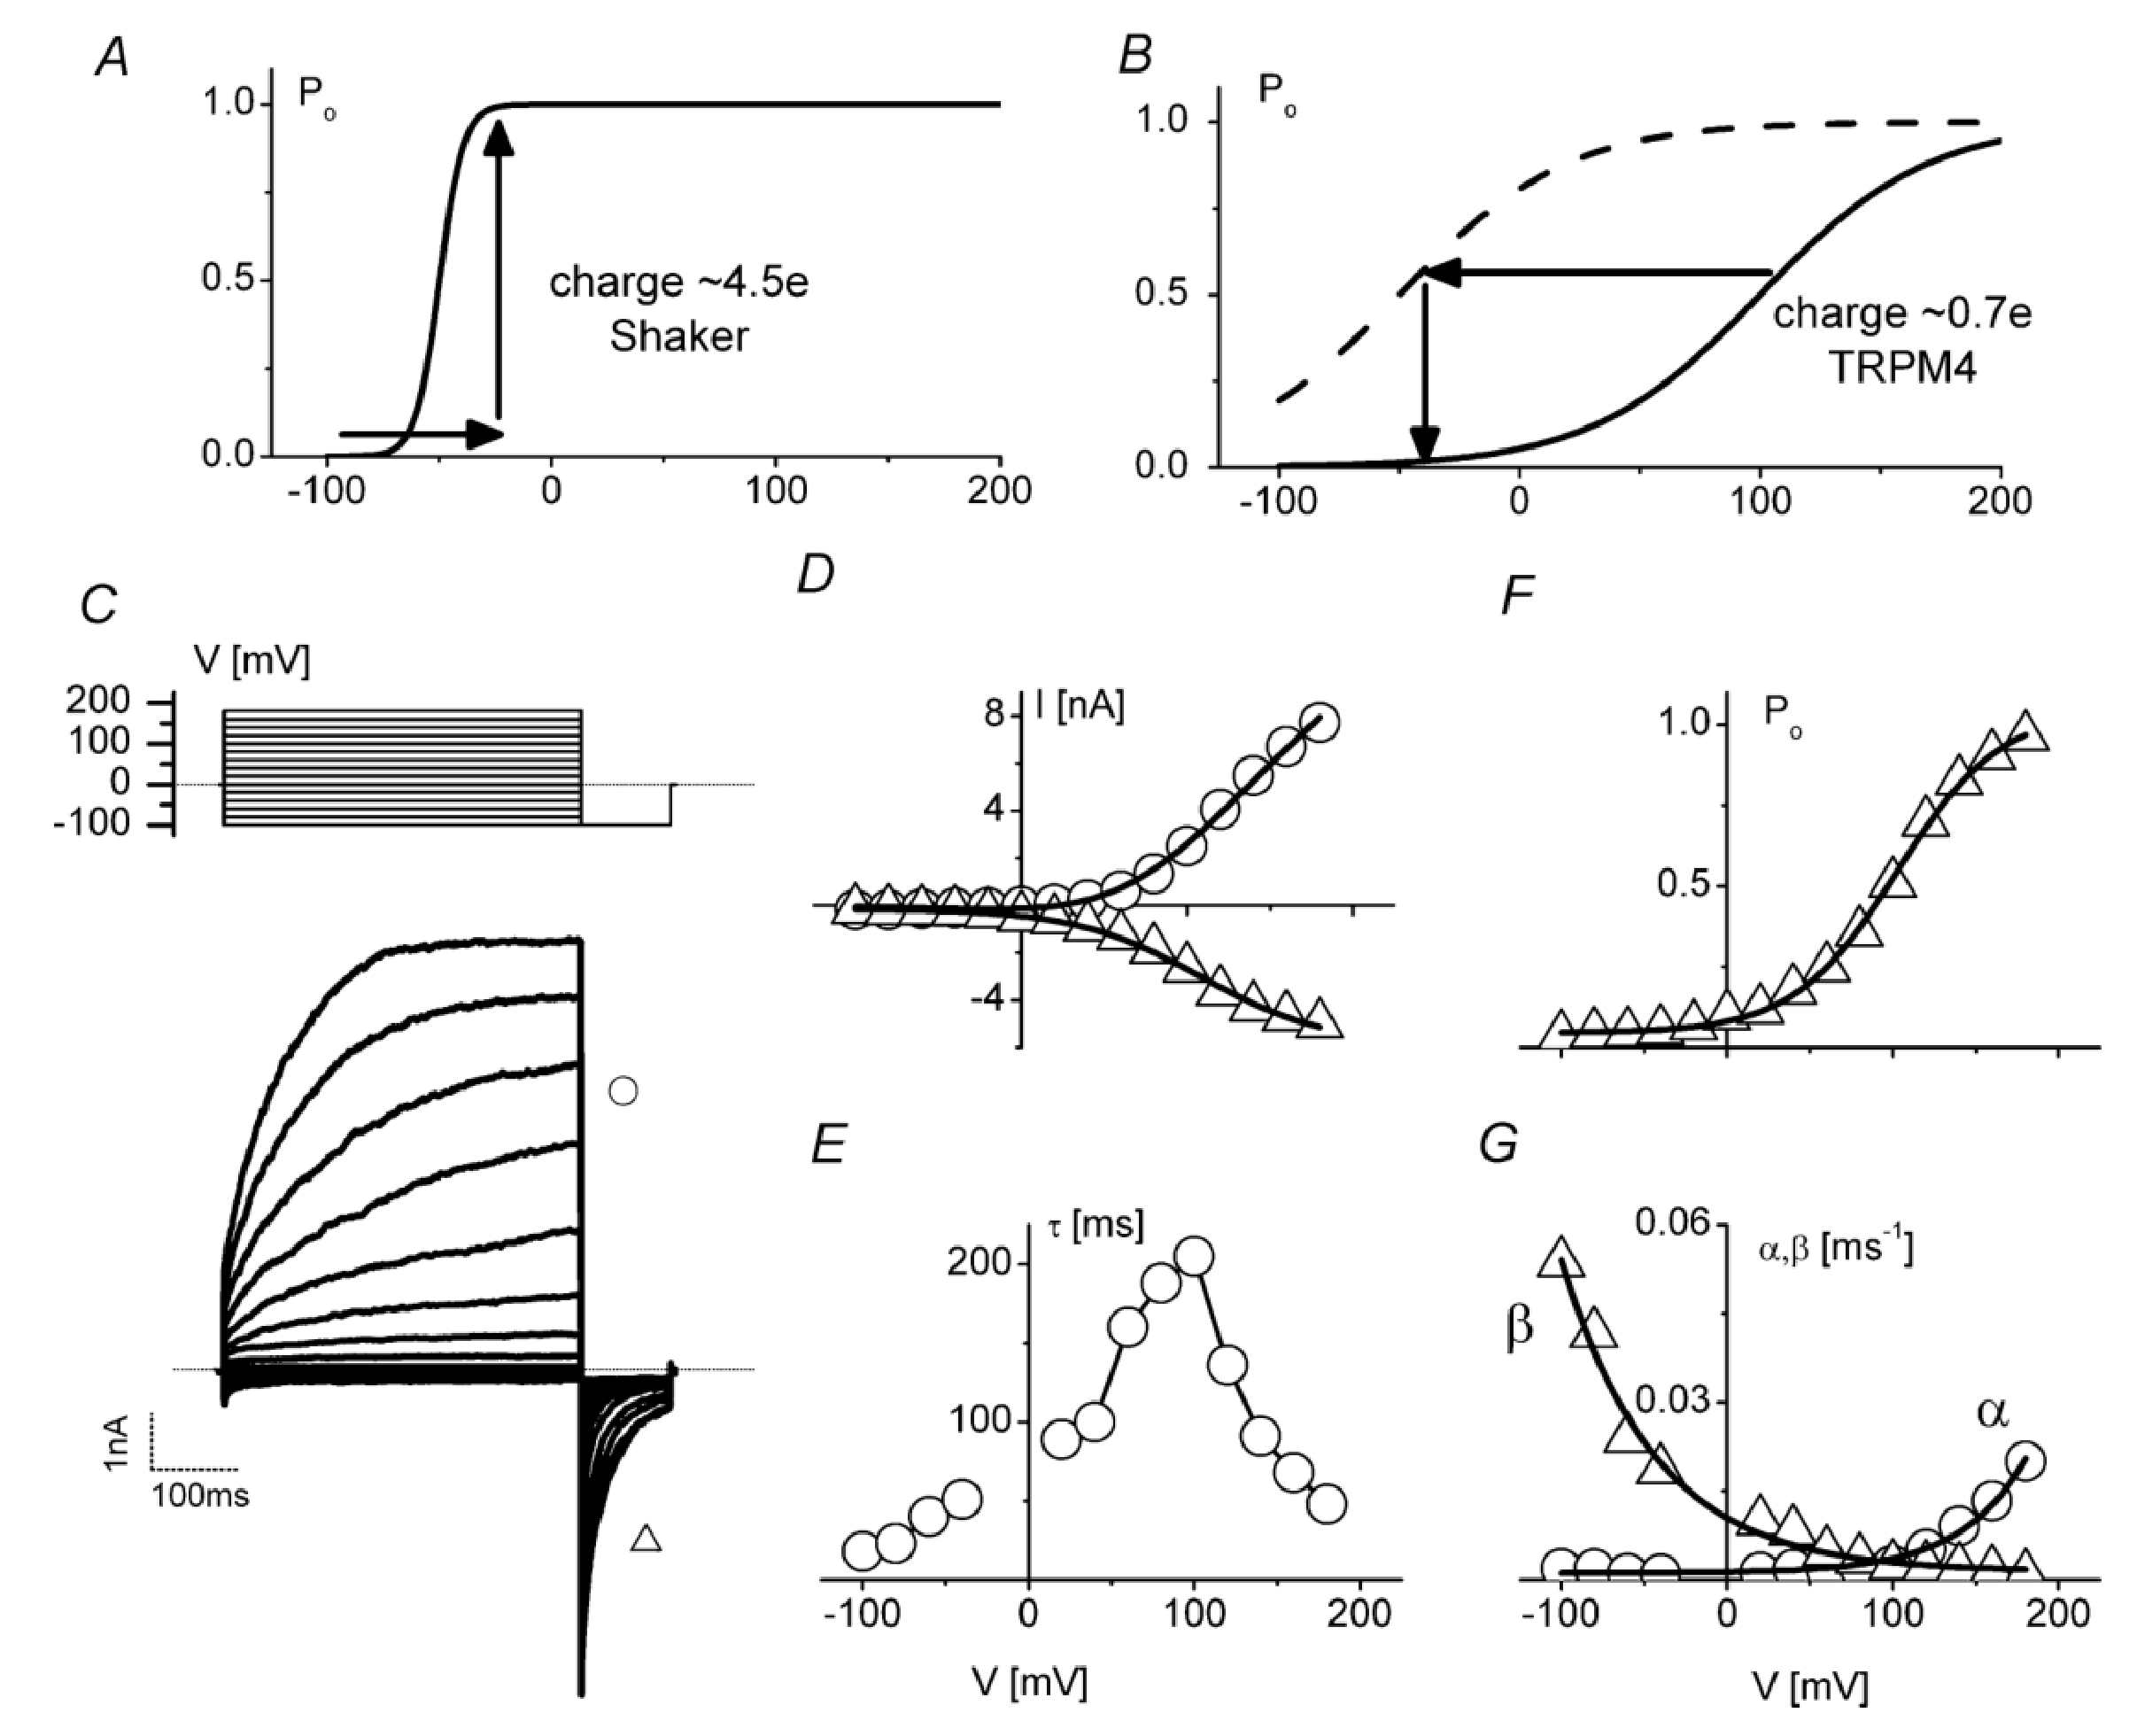
\includegraphics[height=5cm,
    angle=0]{./images/TRP_Vm-dependent.eps}}
  \caption{(A) Activation curve of Shaker $\K$ channel. (B) Activation curve of
  TRP.}
  \label{fig:TRP_Vm}
\end{figure}



\section{Icrac (calcium-release activated calcium current: CRAC)}
\label{sec:Icrac}
\label{sec:CRAC}

Icrac was shown to be a highly Ca2+ selective current, such that the
current-voltage relationship is highly inwardly rectifying with a positive
reversal potential. This current is highly selective for Ca2+ and exhibits
strong negative feedback regulation by Ca2+, which apparently occurs in a region
of high Ca2+ concentration close to the inner aspect of the channel.

The current is strongly inwardly rectifying, but as to whether this is a
property of asymmetrical permeability properties or simply a reflection of the
sizable outwardly directed calcium gradient cannot be experimentally determined.
However, in the complete absence of divalent cations, the channel passes
monovalent cations indiscriminately and loses its property of inward
rectification.

As is the case for other Ca2+-selective channels, Ca2+ both blocks as well as
permeates the channels such that severe reduction of external divalent cations
produces larger inward Na+ currents (Hoth \& Penner, 1993).

Perhaps one of the most interesting properties of the CRAC channels is their
apparent extremely small unitary current, estimated on the basis of noise
analysis to be of the order of a few fA.
Hoth and Penner were not able to detect single channel events by conventional
patch-clamp techniques, and their size was estimated later by use of noise
analysis to be of the order of a few tens of fS (Zweifach \& Lewis, 1993)

\section{}

This second type of capacitative calcium entry current has been observed in
endothelial cells and A431 cells.
The channels are activated by $\Ca$ store depletion, but can also be activated
directly by IP3.
Expression of type 3 IP3 receptor in Xenopus oocytes specifically augments Ca2+
entry, without affecting Ca2+ release, suggesting that the type 3 IP3 receptor
can function in the plasma membrane as a capacitative calcium entry channel.

In these cell types, a divalent cation selective current has been described but,
unlike Icrac the current is associated with identifiable single channel openings
with conductance of the order of 2-10 pS.

These channels also differ from those
underlying Icrac in that they are comparably permeable to both
Ba2+ and Ca2+.


However, they also differ from one another in that the A431 cell channels appear
more permeable to Ba2+ than to Ca2+,(39) while the channels in endothelial cells
appear slightly more permeable to Ca2+.
Perhaps most significantly, in both cell types it appears that these same single
channels can be directly activated by IP3.

\section{Icranc}

Krause et al.(44) have described a nonselective
cation current in mouse pancreatic acinar cells that is activated
by intracellular store depletion, designated Icranc for
calcium release-activated nonselective cation current.

Single channels of the order of 50 pS were associated with this current.

Pharmacologically, it is distinct from Icrac or from the current in endothelial
cells (or from any know capacitative calcium entry mechanisms for that matter)
in that it is not inhibited by La3+ or Gd3+ but is blocked by flufenamic acid or
genestein.






%%% Local Variables: 
%%% mode: latex
%%% TeX-master: "thermo-stat"
%%% End: 





